
\documentclass[12pt,oneside]{memoir} 

\usepackage[latinica]{matfmaster} 
\usepackage{listings}
\usepackage{xcolor}
\usepackage{float}


\definecolor{codegreen}{rgb}{0,0.6,0}
\definecolor{codegray}{rgb}{0.5,0.5,0.5}
\definecolor{codepurple}{rgb}{0.58,0,0.82}
\definecolor{backcolour}{rgb}{0.95,0.95,0.92}

\lstdefinestyle{mystyle}{
    backgroundcolor=\color{backcolour},   
    commentstyle=\color{codegreen},
    keywordstyle=\color{magenta},
    numberstyle=\tiny\color{codegray},
    stringstyle=\color{codepurple},
    basicstyle=\ttfamily\footnotesize,
    breakatwhitespace=false,         
    breaklines=true,                 
    captionpos=b,                    
    keepspaces=true,                 
    numbers=left,                    
    numbersep=5pt,                  
    showspaces=false,                
    showstringspaces=false,
    showtabs=false,                  
    tabsize=2
}

\lstset{style=mystyle}

% \usepackage[biblatex]{matfmaster}
% \bib{thesis}

% Datoteka sa literaturom u BibTex tj. BibLaTeX/Biber formatu
\bib{thesis}

% Ime kandidata na srpskom jeziku (u odabranom pismu)
\autor{Vojkan Cvijović}
% Naslov teze na srpskom jeziku (u odabranom pismu)
\naslov{Razvoj skalabilnih veb servisa na arhitekturi bez servera}
% Godina u kojoj je teza predana komisiji
\godina{2022}
% Ime i afilijacija mentora (u odabranom pismu)
\mentor{prof. dr Aleksandar \textsc{Kartelj}, docent\\ Univerzitet u Beogradu, Matematički fakultet}
% Ime i afilijacija prvog člana komisije (u odabranom pismu)
\komisijaA{prof. dr Saša \textsc{Malkov}, vanredni profesor\\ Univerzitet u Beogradu, Matematički fakultet}
% Ime i afilijacija drugog člana komisije (u odabranom pismu)
\komisijaB{prof. dr Vladimir \textsc{Filipović}, redovni profesor\\ Univerzitet u Beogradu, Matematički fakultet}


% Apstrakt na srpskom jeziku (u odabranom pismu)
\apstr{%
U ovom radu će biti predstavljen razvoj skalabilnog veb servisa zasnovanog na arhitekturi bez servera. Za razvoj veb servisa koristiće se NodeJs programski jezik pomoću kojega ćemo napisati funkcije za AWS Lambda servis. Za bazu podataka koristiće se AWS DynamoDb servis. Kôd će biti postavljen na veb servis putem serverless alata. Za autentifikaciju i autorizaciju koristiće se AWS servis pod nazivom AWS Cognito. Za razvoj android mobilne aplikacije koristiće se programski jezik Kotlin.
}

% Ključne reči na srpskom jeziku (u odabranom pismu)
\kljucnereci{veb servisi, lambda, arhitektura bez servera, android}

\begin{document}
% ==============================================================================
% Uvodni deo teze
\frontmatter
% ==============================================================================
% Naslovna strana
\naslovna
% Strana sa podacima o mentoru i članovima komisije
\komisija
% Strana sa posvetom (u odabranom pismu)
\posveta{Mami, tati i dedi}
% Strana sa podacima o disertaciji na srpskom jeziku
\apstrakt
% Sadržaj teze
\tableofcontents*

% ==============================================================================
% Glavni deo teze
\mainmatter
% ==============================================================================

% ------------------------------------------------------------------------------
\chapter{Uvod}
% ------------------------------------------------------------------------------

\section{Motivacija}
Popularnost računarstva u oblaku raste iz godine u godinu. Računarstvo u oblaku oslobađa klijenta potrebe da poseduje hardver i pruža mogućnost iznamljivanja servera o čijem hardveru i dostupnosti se stara pružalac usluge (engl. cloud provider). Ranije su kompanije morale da kupe ili zakupe određeni server sa pratećim hardverom. U slučaju kupovine morali su i da obezbede adekvatno mesto da takve uređaje. U slučaju da im obim posla poraste, nije postojao lak način da prošire svoje kapacitete. Ovaj način upravljanja je zahtevao i angažovanje dodatnog osoblja koje bi radilo na održavanju takvih uređaja. U slučaju iznamljivanja servera zahteva se određeni nivo upravljanja operativnim sistemom i ostalim softverom na sistemu. Korisnik koji iznajmljuje mora da se stara o održavanju samog sistema, ažuriranju verzija kako paketa tako i samog operativnog sistema. Ovaj scenario se pokazao kao otežavajuci faktor na projektima, pogotovu u kompanijama koje nemaju dovoljno ljudskih resursa i znanja iz domena održavanja. Dodatni otežavajuci faktor je nemogućnost prilagođavanja promenama zahteva opterećenosti samog servera. 

Sa arhitekturom bez servera (engl. serverless architecture) klijent ne poseduje konkretne fizičke resurse već po potrebi koristi deo resursa u skladu sa svojim potrebama. Klijent se na taj način fokusira isključivo na ciljanu aplikaciju. Pružalac usluge se stara o okruženju, o hardveru, operativnom sistemu virtuelnih mašina i upravljanju drugim serverskim softverom. Kôd se obično pokreće unutar kontejnera koji ne čuvaju stanja (engl. stateless container) i koji može biti aktiviran raznim događajima uključujući HTTP zahteve, postavljanje datoteke na server, događaje iz baze podataka, itd.


% ------------------------------------------------------------------------------


\section{Virtuelizacija}
Virtuelizacija se odnosi na apstrakciju neke fizičke kompotente u logičku komponentu. Virtuelizacija je ključna za funkcionisanje računarstva u oblaku. Ona omogućava pružaocima usluga da svojim klijentima brzo omoguće izolovan servis. Po definiciji virtuelna mašina može da virtuelizuje sve hardverske komponente, ukljucujući procesor, memorijski prostor i mrežnu organizaciju \cite{ve}. Monitor virtuelne mašine je softver koji spaja virtuelnu mašinu i server na kome se nalazi virtuelna mašina. Jos je poznat i kao hipervizor. Računar na kojem hipervizor pokreće jednu ili više virtuelnih mašina naziva se domaćin (engl. host) mašina, a svaka virtualna mašina se naziva gostujuća (engl. guest) mašina. Hipervizor dolazi u dva oblika. Kao sloj između serverskom operativnog sistema i gostujuće virtuelne mašine ili virtuelne mašine i samog hardvera \cite{ve}. Poslednji koriste operativni sistemi poput Windows i Linux operativnog sistema. Razlikuju se dve vrste virtuelizacije, virtuelizaciju zasnovanu na hipervizoru i virtuelizaciju zasnovanu na kontejnerima.
 
Velike kompanije poput Google, Amazon i Microsoft imaju svoje centre podataka u kojima su smešteni serveri velike snage. Kako je prateći Murov zakon (engl. Moor's Law) hardverska snaga rasla tako je model jedan server, jedna aplikacija zastarevao. Takvi serveri su imali slabu iskorišćenost. Virtuelizacija omogućava bolju iskorišćenost servera. Ideja virtuelizacije nije nova. Još su se u šezdesetim IBM koristili mejnfrejm (engl. mainframe) računari sa virtuelnim okruženjima. Virtuelizacija je omogućila grupisanje više fizičkih mašina u manji broj servera koji bi dalje pokretali veći broj virtuelnih mašina i samim tim podigli iskorišćenost servera. Što je bolja iskorišćenost servera to je manji broj servera potreban u sali a samim tim i manji su troskovi za njihovo održavanje, manje zaposlenih mora da ih održava i manje energije se utroši na njihovo hlađenje. Pored mogućnosti grupisanja (engl. consolidation), virtuelizaija je omogućila i mogućnost zadržavanja (engl. containment) aplikacija na postojećoj virtuelnoj infrastrukturi. To je kompanijama omogućilo lak prenos virtuelnih mašina sa jednog hardvera na drugi. Administratori mogu da zaustave virtuelnu mašinu u svakom trenutku i da je lako oporave na prethodno ispravno stanje. Računarstvo u oblaku bi bilo nemoguće bez virtuelizacije kako ona omogućava da se veliki centri podataka transformišu u skalabilne i lako dostupne resurse. Virtuelizacija omogućava transformaciju centara u virtuelne centre podataka što dalje olakšava dostavljanje resursa klijentu. Virtuelni centri podataka se dalje organizuju po virtuelnim regionima \cite{ve}.

\subsection{Virtuelizacija zasnovana na hipervizorima}
Hipervizor se može posmatrati kao arbitar resursa. To je softver koji se nalazi između virtuelne mašine i samog fizičkog hardvera kao što se može videti na slici\ref{fig:hipervizor}. Omogućava virtuelnoj mašini da upravlja sa memoriom, da pristupa virtuelnim mrežama za komunikaciju, efikasno korišćenje sve veće memorije kod novijih procesora \cite{ve}. Bez hipervizora svaka virtuelna mašina bi morala direktno da pristupa disku što bi napravilo problem ako bi jos jedna mašina izvršavala paralelno operaciju pristupa disku. Hipervozor se stara da svaka virtuelna mašina može da koristi hardver bez obzira na ostale virtuelne mašine.
\begin{figure}[!ht]
  \centering
  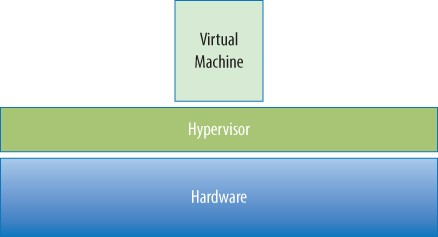
\includegraphics[width=0.7\textwidth]{Slika 1.jpg}
  \caption{Hipervizor\newline[preuzeto iz knjige Virtualization essentials, autora Matthew Portnoy]}
  \label{fig:hipervizor}
\end{figure}
 
Postoje dva tipa hipervizora a to su tip 1 i tip 2. U nastavku rada su predstavljene njihove karakteristike.
 
\subsubsection{Tip 1 hipervizor}
Kao što se može videti na slici\ref{fig:hipervizorTip1}, ovaj tip hipervizora se nalazi se direktno na serverskom hardveru bez operativnog sistema ispod. Direktno komunicira sa hardverom što ga čini mnogo efikasnijim od tipa 2. Ne postoji trošak održavanja operativnog sistema koji bi služio kao posrednik. Pored boljih performansi tip 1 hipervizori su bezbedniji. Virtuelne mašine koje se izvršavaju iznad hipervizora, ne mogu da utiču na hipervizor. One su ograđene u svoj prostor i mogu da izazovu pad samo sopstvene virtuelne mašine. Ostale virtuelne mašine ostaju neometene.
\begin{figure}[!ht]
  \centering
  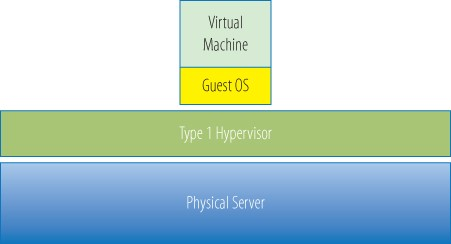
\includegraphics[width=0.7\textwidth]{Slika 2.jpg}
  \caption{Hipervizor tip 1\newline[preuzeto iz knjige Virtualization essentials, autora Matthew Portnoy]}
  \label{fig:hipervizorTip1}
\end{figure}
 
\subsubsection{Tip 2 hipervizor}
Tip 2 hipervizor je zapravo aplikacija koja radi na postojećem operativnom sistemu što se može videti na slici\ref{fig:hipervizorTip2}. Lakši su za instalaciju kako ne zahtevaju veliki obim konfigurisanja. Podešavanja prostora za podatke i mreža su već odrađeni od strane postojećeg oprativnog sistema. Ovaj tip hipervizora može da podržava veliki broj različitih hardverskih komponenti kako su one već podržane od strane operativnog sistema na kome je hipervizor instaliran. Tip 2 hipervizora ima slabiju efikasnost od tipa 1 \cite{ve}. Kako radi sa posrednikom, operativnim sistemom, operacije nisu direktne pa su samim tim i sporije. Svaku operaciju koju virtuelna mašina prosledi hipervizoru, on dalje mora da prosledi operativnom sistemu, koji mora da je pročita i dalje izvrši odgovarajuću operaciju na hardveru. Za razliku od tipa 1 gde ne postoji posrednika i sve operacije se izvršavaju direktno na hardveru. Iz tog razloga je tip 1 efikasniji od tipa 2. 
Ovaj tip hipervizora je takođe manje pouzdan od tipa 1. Kako postoji operativni sistem na kome se hipervizor nalazi, taj operativni sistem je potrebno održavati. Ponekad je potrebno i restartovati operativni sistem da bi se zavrsila instalacija, to dalje prouzrokuje da se sve virtuelne mašine moraju restartovati. Tip 2 hipervizori se obično nalaze na desktop računarima gde korisnici mogu da rade na više različitih virtuelnih mašina, dok se tip 2 nalazi na serverima čiji jedini zadatak je da služe za izvršavanje virtuelnih mašina.

\begin{figure}[!ht]
  \centering
  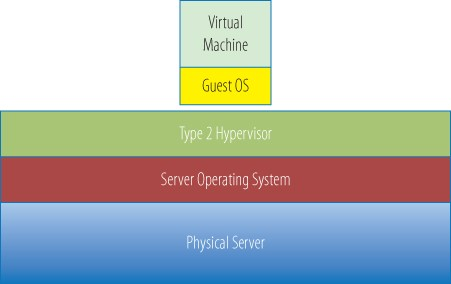
\includegraphics[width=0.7\textwidth]{Slika 3.jpg}
  \caption{Hipervizor tip 2\newline[preuzeto iz knjige Virtualization essentials, autora Matthew Portnoy]}
  \label{fig:hipervizorTip2}
\end{figure}

 
\subsection{Virtuelizacija zasnovana na kontejnerima}

Virtuelizacija zasnovana na kontejnerima se izvršava na nivou operativnog sistema deleći sa njim sistemski kernel. Za razliku od virtuelizacije zasnovane na hipervizoru koja virtuelizuje ceo hardver, virtuelizacija zasnovana na kontejnerima zahteva mnogo manje virtuelizacije. Samim tim sto ne zahteva podizanje celog operativnog sistema prilikom startovanja kontejnera, vreme startovanja je kraće \cite{gswc}. 
 
\begin{figure}[!ht]
  \centering
  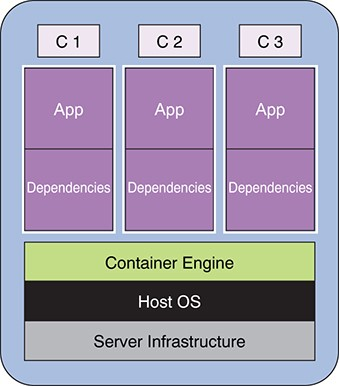
\includegraphics[width=0.7\textwidth]{Slika 4.jpg}
  \caption{Kontejneri\newline[preuzeto iz knjige Microservices and containers, autora Parminder Kocher]}
  \label{fig:kontejneri}
\end{figure}
 
Kao sto se vidi na slici\ref{fig:kontejneri}. Kontejneri omogućavaju izolaciju aplikacije od ostalih aplikacija na serveru. Kontejner može da funkcioniše bez znanja koliko jos kontejnera se izvršava na operativnom sistemu. Svi kontejneri dele isti kernel i odgovornost za to je na strani operativnog sistema. Svaki operativni sistem ima metode za obezbeđivanje izolacije kontejnera. Na Linux operativnom sistemu su to kontrolne grupe (engl. control groups) i prostor imenovanja (engl. namespace). Iz tog razloga može se izvršavati više kontejnera na zadatom hardveru nego virtuelnih mašina \cite{mac}. 

Kontejneri su lakši za izvršavanje kako im ne treba ceo operativni sistem ali virtuelne mašine prižaju bolju izloaciju kako ne dele direktno resurse sa operativnim sistemom. Kontejneri takođe efikasnije koriste hardverske resurse. Ovaj tip kontejnera je jos poznat kao Linux kontejneri (engl. Linux containers) ili LXCs. Postoji još i tip Doker (engl. Docker) kontejnera. Doker je uveo par promena koje su učinile da su kontejneri postali pristupačniji, fleksibilniji i lako prenosni \cite{gswc}. Razlike između LXC i Doker kontejnera:
\begin{enumerate}
  \item Procesi. Kod Linuks kontejnera može imati više procesa dok kod Doker kontejnera može imati samo jedan proces. To može da dovede do problema ukoloko aplikacija zahteva više procesa za izvršavanje.
  \item Skladištenje podataka. Doker kontejneri ne čuvaju stanje (engl. stateless). Potrebno je obezbediti eksterni prostor za čuvanje podataka.
  \item Prenosnost. Kod Linuks kontejnera prenosivost nije garantovana dok je kod Doker kontejnera prenosivost garantovana.
\end{enumerate}

\section{Računarstvo u oblaku}

Računarstvo u oblaku je koristi da bi se opisao skup računara, servisa i resursa koje programeri mogu da koriste prilikom razvoja sistema zasnovanih na vebu. Primeri takvih resursa mogu biti računarski, skladišni prostor, mrežni, aplikativni. Ti resursi se posmatraju kao virtuelni iz razloga ukoliko je potrebno proširiti broj resursa, pružaoci usluga to lako omogućavaju. Klijenti plaćaju samo resurse koje koriste, a na kompanijama koje pružaju usluge iznamljivanja je da se staraju o dostupnosti tih servisa, resursa i o održavanju centara gde se nalaze serverske mašine. Na klijentu ostaje da se fokusira na svoje i potrebe aplikacije \cite{cc}.

%% Nabrajanje?! Formulisati drugacije?
Karakteristike računarstva u oblaku:
\begin{enumerate}
  \item Usluga na zahtev (engl. on-demand service). Korisnik samostalno može odabrati, pokrenuti i konfigurisati računarske resurse. Većina pružalaca usluga naplaćuje korišcenje resursa u zavisnosti od vremena u kojem su bili aktivni.
  \item Široki mrežni pristup (engl. broad network access). Računarski resursi su dostupni preko mreže velike propusne moći i mogu im pristupiti različite klijentske platforme.
  \item Udruživanje resursa (engl. multi-tenancy and resource pooling). Računarski resursi su dizajnirani tako da podržavaju model više zakupljenih jedinica (engl. multi-tenancy model). Time se omogućava da više klijenata deli fizičku infrastrukturu a da su privatnost podataka i bezbednost obezbeđeni. U modelu više zakupljenih jedinica, jedan računarski hardver može opsluživati više klijenata.
  \item Brza elastičnost i skalabilnost (engl. rapid elasticity and scalability). Omogućava da se kreiraju ili unište resursi u sto kraćem vremenskom roku. Resursi mogu da se povećaju (engl. scale-up) ili da se smanje (engl. scale-down) u zavisnosti od klijentskih potreba. Pružaoci usluga nude i opciju automatskog prilagođavanja u skladu sa samim opterećenjem servera (engl. autoscaling).
  \item Izmerena usluga (engl. measured service). Upotreba resursa se može pratiti, proveravati i o njoj se mogu praviti izveštaji pružajući transparentan uvid o uslugama i korisnicima. Klijent plaća računarske resurse koje je koristio.
\end{enumerate}

Kao sto se može videti na slici\ref{fig:servisniModeli}, u zavisnosti od nivoa kontrole infrastrukture koje je dato klijentu, razlikuju se tri servisna modela računarstva u oblaku. U nastvaku rada predstavljene su njihove prednosti i mane.

\begin{figure}[!ht]
  \centering
  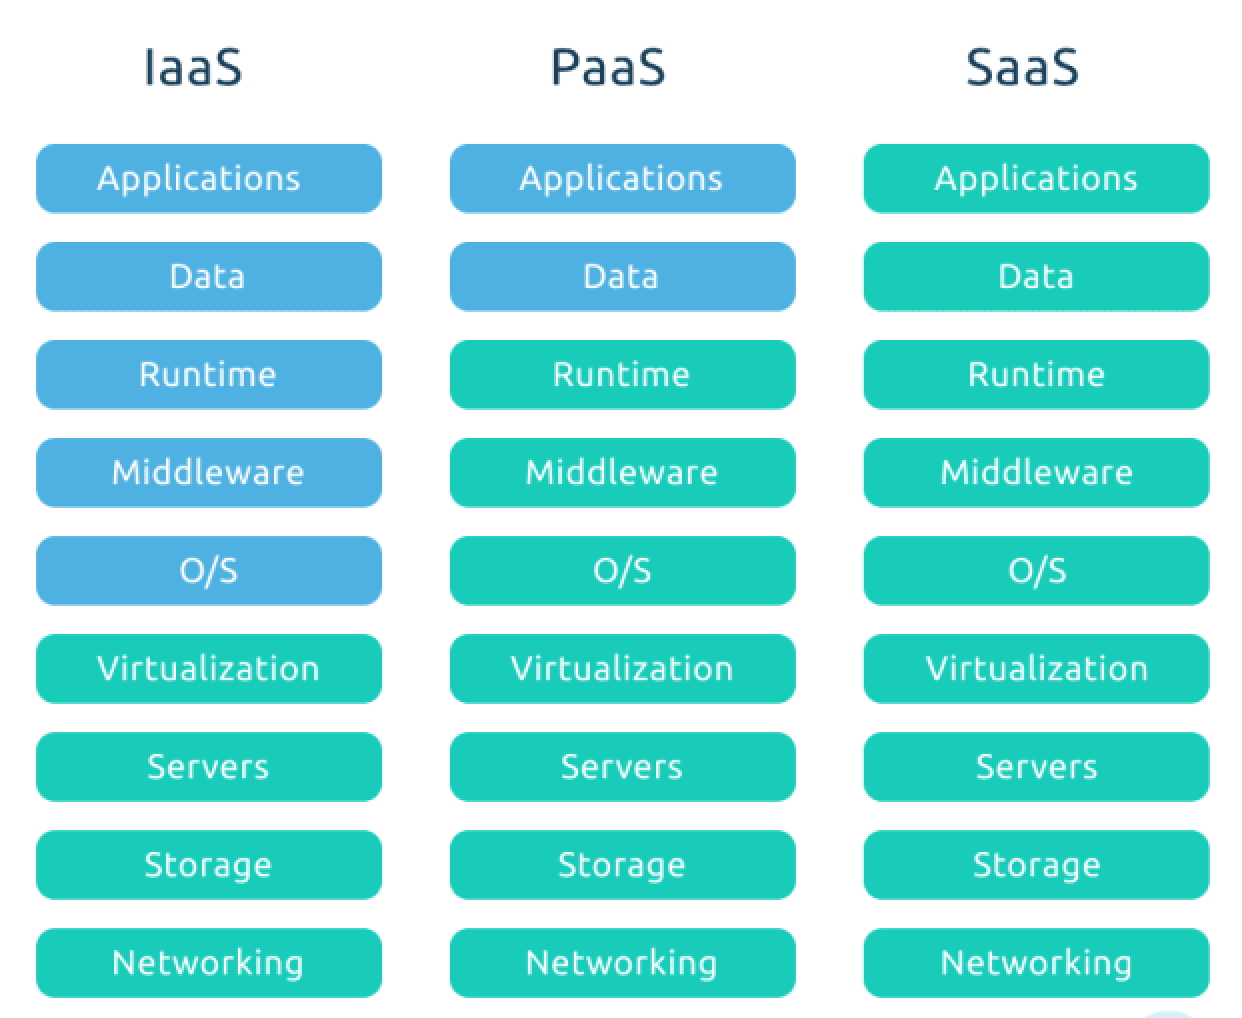
\includegraphics[width=0.7\textwidth]{Slika 5.png}
  \caption{Servisni modeli\newline[preuzeto sa sajta https://dev.to]}
  \label{fig:servisniModeli}
\end{figure}
 
\subsection{Infrastruktura kao servis}

U ovom modelu sva kontrola računarskog hardvera je data na raspolaganje klijentu. Pružalac usluga se stara u hardveru i pratećoj infrastrukturi dok je klijentu predata potpuna kontrola nad operativnim sistemom i njegovim komponentama. Klijent mora sam da se stara o održavanju sistema, ažuriranju softvera, praćenju opterećenosti računarskih resursa poput procesora i memorije. Klijentu je prepušteno da se sam stara o pravljenju sigurnosnih kopija same mašine za slučaj otkazivanja neke komponente. Ovaj model može biti izazovan za manje firme koje ne mogu da priušte tim zaposlenih koji će se baviti održavanjem virtuelnih mašina. Model je predviđen za velike kompanije koje žele punu kontrolu nad svojim resursima a ne žele da ih drže u svojim centrima podataka \cite{cc}. Komercijalni primeri modela infrstruktura kao servis su Amazon Elastic Compute Cloud, Google Compute Engine i Azure Virtual Machines. %-> Kako ovo navesti? 

 
\subsection{Platforma kao servis}
U ovom modelu klijentu nije omogućeno upravljanje infrastrukturom ukljucujući operativnim sistemom, mrežnim podešavanja, prostorom za skladištenje podataka. O operativnom sistemu, pratećim komponentama i njihovom održavanju se stara pružalac usluga. Pružalac usluga klijentu nudi skup softverskih i hardverskih alata koji treba da mu pomognu u upravljanju aplikaciom. Korisniku nije omogućeno upravljanje infrastrukturom ali omogućeno mu je da kroz konfiguraciju prilagodi infrastrukturu u određenoj meri. U zavisnosti od potreba klijenti se mogu opredeliti za rešenja bazirana na Windows ili Linux operativnom sistemu. Korisnik može imati poteškoće prilikom integrisanja sa postojećim servisima iz svog centra podataka. Takođe postoji opasnost od zaključavanja kod konkretnog pružaoca usluga(engl. vendor locking) posle čega će migracija biti otežana \cite{cc}. Primeri komercijalnih rešenja su Heroku, Google App Engine, WordPress i AWS Elastic Beanstalk. %-> Kako ovo navesti? 


\subsection{Softver kao servis}
U ovom modelu klijentu se daje na raspolaganje pristup softveru uglavnom preko veb pregledača. Sam softver, dodatni alati i korisnički podaci se nalaze u oblaku (engl. cloud). Zato što se svi resursi nalaze kod pružaoca usluga, celo rešenje se može lako skalirati. Pružalac usluga se stara i o samom hardveru i operativnom sistemu. Plaćanje se uglavnom vrši prema broju korisnika aplikacija. Korisnik može da podesi aplikaciju kroz konfiguracije koje mu je omogućio pružalac usluga. Aplikacije se mogu koristiti i bez prethodnog konfigurisanja, kao npr aplikacije za dopisivanje, dok neke aplikacije zahtevaju konfigurisanje sa korisničke strane pre nego sto se mogu koristiti. Neki primeri komercijalnih rešenja su Slack, ServiceNow, Jira, OneDrive. %-> Kako ovo navesti? 


\subsection{Tipovi računarstva u oblaku} % ->(engl. Cloud deployment model -> kako prevesti)
 
Postoje tri tipa računarstva u oblaku. U zavisnosti od potreba, korisnik se može opredeliti za javni, privatni ili hibridni tip računarstva u oblaku. U nastavku rada predstavljene su njihove karakteristike.


\subsubsection{Javni oblak} % treba li mi subsubsection?
Javni oblak je u vlasništvu pružalaca usluga i dostupan je svima preko interneta. Ovaj tip omogućava korisniku da zakupi resurse od pružalaca usluga. Pružalac usluga je zadužen da kreiranje i održavanje računarskih resursa. Računarski resursi se mogu zakupiti na bilo kojoj geografskoj lokaciji. Pružaoci usluga garantuju određen nivo pouzdanosti resursa. Prema izveštaju Alijanse za bezbednost podataka u oblaku (engl. Cloud Security Alliance, CSA) 89\% organizacija čuva osetljive podatke u oblaku, od toga 67\% čuva osetljive podatke u javnom oblaku. U izveštaju je još navedeno da se 44\% organizacija ne oseća pouzdanim da mogu da zaštite podatke u javnom oblaku pored svih mehanizama koje pružaoci usluga obezbeđuju. Prema tome izveštaj preporučuje je potrebno staviti akcenat na adekvatne mere zaštite podataka, npr enkripciju istih \cite{csa}.
% da li je navedeno dobro?
%https://cloudsecurityalliance.org/artifacts/sensitive-data-in-the-cloud/

 
\subsubsection{Privatni oblak}
Privatni oblak je napravljen isključivo za upotrebu jednog klijenta. Rezervisan centar podataka za tog klijenta, koji može biti unutar organizacije ili iznajmljen od pružaoca usluga. Pruža veći nivo kontrole pristupa za razliku od javnog oblaka. Iako košta više od javnog oblaka, velike firme ga koriste da bi podigle nivo bezbednosti i oblikovale računarske resurse u skladu sa njihovim potrebama. Prema izveštaju CSA od 89\% organizacija koje čuvaju osetljive podatke u oblaku, 45\% njih čuva podatke na privatnom oblaku \cite{csa}.
% hostovan? Formulisati drugacije?
 
\subsubsection{Hibridni oblak}
Predstavlja spoj javnog i privatnog oblaka. Sastavljeni su od dva ili više oblaka, barem jednog privatnog i barem jednog javnog. Privatni i javni oblaci su povezani u jedan entitet standardizovanim tehnologijama za povezivanje. Privatni oblak se može proširiti resursima iz javnog oblaka čime se postiže bolja otpornost na velika opterećenja. Potrebno je odrediti koji resursi se nalaze u privatnom a koji u javnom oblaku. Postoji mogućnost pojave uskog grla (engl. bottleneck) između privatnog i javnog oblaka.


\section{Projektni uzorci softverske arhitekture}
Arhitektura bez servera omogućava skaliranje pojedinačnih komponenti što može uticati na opštu arhitekturu softvera. Da bi smo u potpunosti iskoristili bonuse arhitekture bez servera, arhitektura softvera mora biti adekvatna. U arhitekturi bez servera svaka komponenta, funkcija ili svaki servis moraju biti lagani (engl. lightweight) i agilni. Funkcije se skaliraju pa je obavezno da imaju kratko vreme startovanja. U ovom poglavnju se razmatraju karakteristike monolitne i mikroservisne arhitekture. Na slici\ref{fig:arhitekturniProjektniUzorci} se može videti razlika između monolitne i mikroservisne arhitekture na primeru veb (engl. web) aplikacije.

\begin{figure}[!ht]
  \centering
  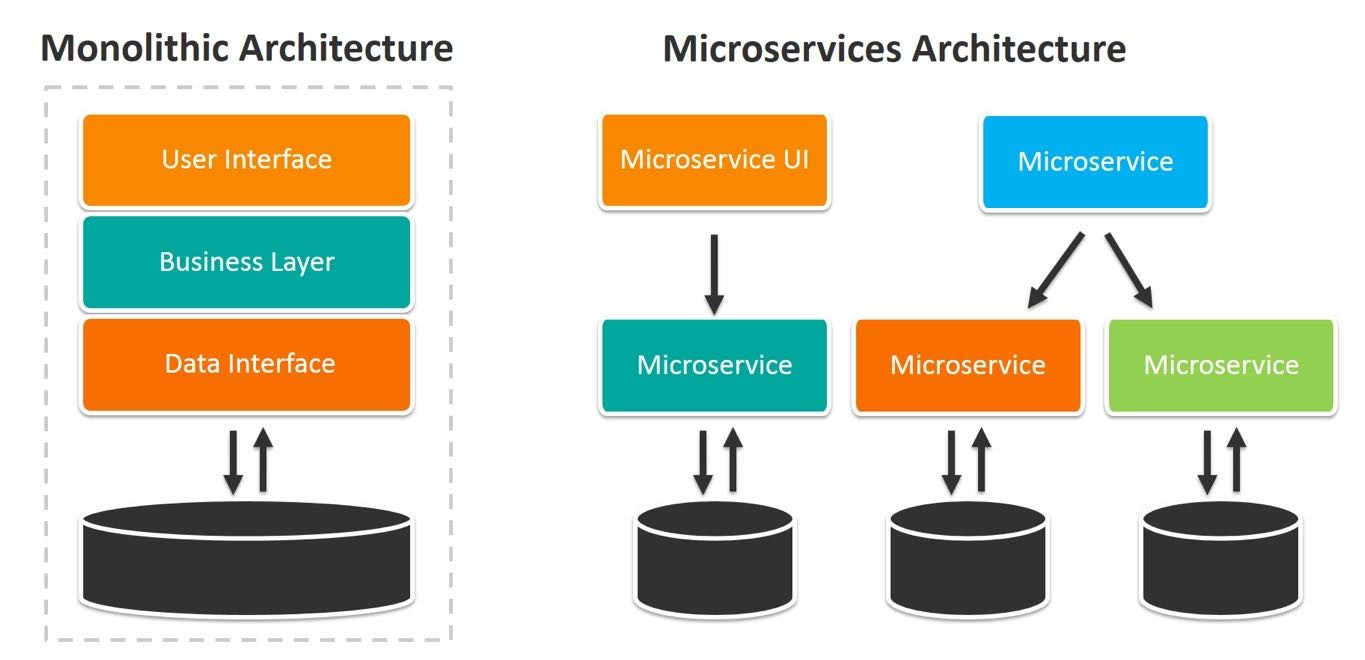
\includegraphics[width=0.7\textwidth]{Slika 6.jpg}
  \caption{Primer veb aplikacije u monolitnoj i mikroservisnoj arhitekturi\newline[preuzeto sa sajta https://www.suse]}
  \label{fig:arhitekturniProjektniUzorci}
\end{figure}

\subsection{Monolitna arhitektura}
Monolitna arhitektura predstavlja tradicionalni model izrade softvera. Softver se sastoji od jedne celine koja je nezavisna od drugih aplikacija ili servisa. Kod monolitnih aplikacija se razlikuju tri tipa \cite{bm}:
%(Building Microservices, 2nd Edition, What Are Microservices?, The Monolith)
\begin{enumerate}
  \item Monolit sadržan od jednog procesa(engl. single-process monolith). Ceo kôd se izvršava u jednom procesu. Može postojati i više instanci ali suštinski ceo kôd se nalazi u jednom procesu. 
  \item Modularni monolit. Predstavlja proširenje monolita zasnovanog na jednom procesu. Sastoji se od više logički odvojenih modula koji ne mogu da funkcionišu samostalno van grupe modula. Čest problem kod modularnih monolita je to što podaci u bazi nisu dekomponovani kao sto što je kôd podeljen u odvojene module.
  \item Distribuirani monolit. Sistem koji se sastoji od više međusobno usko povezanih servisa. Svim servisima se mora u isto vreme odraditi isporučivanje koda(engl. deployment). Ovakvi sistemi imaju sve mane distriburanih sistema i jedno procesnih monolita bez i jedne prednosti pomenutih.
\end{enumerate}
 
Monolitna arhitektura ima svoje prednosti. Lako isporučivanje koda (engl. deployment) kako se kôd isporučuje kao jedna celina čime se ceo proces značajno uprošćava. Performanse sistema, ceo kôd se izvršava kao deo jedne celine pa nema potrebe za pravljenjem HTTP (engl. The Hypertext Transfer Protocol) poziva unutar same aplikacije. Time se ubrzava ceo proces pošto HTTP zahtevi mogu da se prekinu pa je ih potrebno ograditi sa mehanizmom za ponavljanje. Lakse debagovanje (engl. debugging) i nalaženje bagova. Olakšano je testiranje celog sistema za razliku od distribuiranih sistema. Prednosti monolitne arhitekture najviše dolaze do izražaja kod manjih aplikacija \cite{bm}.
 
Monolitna arhitektura ima i svoje mane. Ne mogu da se skaliraju pojedinačne komponente sistema u slučaju modularnog monolita. Ukoliko je jedna komponenta opterećenija od ostalih, ne može se samo ona klonirati već mora ceo monolit. Komponente monolitne aplikacije su usko povezane (eng tightly coupled) tako da problem u jednoj komponenti može dovesti do pada druge komponente. Naročito je problematično za velike timove koji razvijaju istu monolitnu aplikaciju paralelno, promene koje je uveo jedan tim mogu da dovedu do greške na funkcionalnostima koje je radio drugi tim. Sužen izbor tehnologija, sve komponente monolitne ahritekture moraju biti napisane koristeći isti kôd. Migracija na novije tehnologije može biti izazovna kako zahteva promenu u celom projektu. Održavanje može biti otežano. Velike monolitne aplikacije su komplikovane za održavanje i mogu da smanje produktivnost na projektu. Male promene u kodu zahtevaju isporučivanje cele aplikacije. Monolitna arhitektura može biti dobar izbor u odrđenim trenucima ipak za aplikacije zasnovane na arhitekturi bez servera (engl. serverless) nije najbolji izbor posto one ostvaruju najviše benefita ukoliko je aplikacija organizovana u više manjih odvojenih servisa \cite{sa}.
%(Serverless Architectures on AWS, Second Edition,  Going Serverless, Understanding serverless architectures)

\subsection{Mikroservisna arhitektura}
Mikroservisna ahritektura podrazumeva da je aplikacija podeljena na više nezavisnih servisa prema domenu poslovanja (engl. business domain) \cite{bm}. Svaki servis enkapsulira neke funkcionalnosti i omogućava drugim servisima da ih koriste preko mreže. Mikroservisna arhitektura izbegava deljenje baze podataka tako da svaki servis koji ima potrebu za bazom podataka, ima svoju instancu baze podataka. 

Kod mikroservisne arhitekture je olakšano održavanje koda. Manjim timovima mogu biti dodeljeni pojedinačni servisi na koje se oni fokusiraju. Lakše je održavanje manjih logičkih celina, lakše se nalaze greške (engl. bugs). Veća je otpornost sistema na povećanje dolaznog saobraćaja. Ukoliko je jedan servis opterećeniji od ostalih, može se skalirati (engl. scale). Kako su servisi nezavisni, dodavanje jos jedne instance servisa ne može uticati negativno na ceo sistem. Sistemi dizarnirani po modelu mikroservisne arhitekture imaju veću otpornost na greške u poređenju sa monolitnom arhitekturom. Ukoliko dođe do pada jednog servisa, ostali servisi mogu da nastave da funkcionišu. Kôd na servisima može biti isporučen nezavisno od ostalih servisa. Ukoliko problem nastane posle isporučivanja koda, servis može biti izolovan i vraćen na stariju, ispravnu verziju. Pruža veći izbor tehnologija. Kako se sistem sastoji od više nezavisnih servisa, svaki servis može biti napisan u drugom programskom jeziku. Za servis je vazno da svoju funkcionalnost omogućava preko interfejsa bez obzira u kojoj tehnologiji se sam servis izvršava.
% Zaključak pasusa?

Mikroservisna arhitektura uvodi dodatnu kompleksnost prilikom dizajniranja projekta. Potrebno je napraviti pouzdan komunikacioni mehanizam između servisa koji će biti otporan na greške u mreži. Kako se uglavnom koriste HTTP zahtevi za komunikaciju, potrebno je napraviti mehanizme za ponavljanje zahteva. Potrebno je razlikovati idempotentne (engl. idempotent) i neidempotentne (engl. non-idempotent) zahteve. Kako je sistem podeljen na više manjih servisa, isporučivanje koda je komplikovaniji proces. Takođe svaki servis se mora pratiti sa alatima za monitoring i obezbediti bezbednosnim mehanizmima. Teže je debagovanje i nalaženje grešaka. Glavni izazov kod mikroservisne arhitekture je kako se odlučiti na podelu sistema na manje servise \cite{bm}.
%(Building Microservices, 2nd Edition, How To Model Microservices)

\chapter{Računarstvo bez servera}
\label{chp:razrada}

Računarstvom bez servera (engl. serverless computing) je može nazvati svaki softver (engl. software) koji se isporučuje korisniku kao usluga i naplaćuje se samo kada se koristi\cite{sa}. Softver kao usluga je servisni modeli računarstva u oblaku koji podrazumeva da svako ko koristi softver, koristi ga kroz veb interfejs. Neki primeri softvera kao usluga su Office365 i GoogleMaps. Prateća infrastruktura je sakrivena od korisnika, sve konfiguracije su korisniku dostupne proz veb interfejs. Kreiranje, održavanje, upravljanje prateće infrastrukture je dužnost pružaoca usluga i korisnik može da se fokusira na razvoj sopstvene aplikacije. Osobina da se softver naplaćuje samo kada se koristi označava da korisnik nema troskove dok priprema i konfiguriše softver, troškovi se računaju tek kada softver počne da se koristi.

Početak bez serverskog računarsva se vezuje za pojavu platforme Zimki (engl. Zimki) 2006. godine koju je razvilo odeljenje kompanije Canon (engl. Canon, Inc). Zatim 2008. godine Google objavljuje svoju verziju platforme za bez serversko računarstvo pod nazivom Google App Engine. Mnogim programerima ova platforma je bila previše restriktivna i nije se smatrala kao rešenje spremno za produkciju \cite{ls}. Iako je objavljena 2008. godine, tek 2011. godine izlazi zvanična verzija. Ona je omogućavala samo izvršavanje Python skripti. Termin bez servera (engl. serverless) je prvi put uveden 2012. godine u članku koji je napisao Ken From (engl. Ken Fromm) na sajtu Iron.io \cite{wtfosaais}. Kompanija Amazon lansira svoju verziju platforme pod nazivom AWS Lambda 2015. godine. Zatim kompanija Google izbacuje svoj servis za bez serversko računarstvo Google Cloud Functions 2016. Iste godine Microsoft objavljuje Microsoft Azure Cloud Functions. Postoje i primeri platformi otvorenog koda (engl. open source) koji mogu da se izvršavaju u privatnom oblaku. Neki primeri su Kubeless, OpenWhisk, Fission, OpenFaaS, and Knative \cite{ws}.

\section{Bezserverski modeli računarstva u oblaku}
Postoje dva bezserverska modela računarstva u oblaku (engl. Serverless cloud computing models). Zadnji kraj (engl. backend) kao usluga (engl. Backend as a Service - BaaS) i funkcija kao usluga (engl. Function as a Service - FaaS). U nastavku se razmatraju njihove specifičnosti.

\subsection{Zadnji kraj kao usluga}

%third-party? prevod
%bekend, prevod?
Zadnji kraj kao usluga se odnosi na usluge trećih lica (engl. third-party) koje su dostupne preko aplikativnog interfejsa (engl. Application Programming Interface - API) i koriste se da bi upotpunili ili zamenili neke funkcionalnosti u aplikaciji. Na primer pružalac usluga može omogućiti servis za autentifikaciju, mehanizam dodatne enkripcije ili pristup bazama podataka u oblaku. Ovi servisi se uglavnom koriste kod jednostavnijih veb aplikacije ili mobilnih aplikacija za autentifikaciju \cite{wis} \cite{bsa}. Neki od komercijalnih primera su AWS Amplify i Firebase \cite{baasp}.

\subsection{Funkcija kao usluga}
Funkcija kao usluga omogućava da se kôd isporuči pružaocu usluga a dalje pružalac usluga se stara da se taj kôd izvršava kao deo funkcije. Ove funkcije se pokreću na određeni dolazni događaj koji je zadat kada je i napravljena funkcija. Događaji mogu biti HTTP (engl. HyperText Transfer Protocol) pozivi, poruke, događaj koji se napravi kada se na primer fajl okači na AWS S3 servis, upis u bazu. Na primer, korisnik može da konfiguriše funkciju da kada se okači slika na AWS S3 servis, funkcija se aktivira i promeni format slike u adekvatni format. Pružalac usluga vodi računa o skaliranju infrastrukture pa korisniku deluje kao da server ni ne postoji. 

Funkcije se izvršavaju u kontejnerima koji ne čuvaju stanje i koji su aktivni koliko je aktivna i sama funkcija. Kontejneri ne čuvaju stanje između izvršavanja funkcija pa se sve promene moraju čuvati na nekom drugom servisu, npr u bazi podataka. Pružalac usluga odrđuje koliko dugo kontejneri rade nakon sto se izvršavanje funkcije završi. Klijentu je omogućeno da prosledi i konfiguracioni fajl prilikom isporučivanja koda funkcija. Klijent može da odredi na koje događaje će koje funkcije da se pokreću ili da postavi promenljive po okruženjima (engl. environment variables). Funkcija ostaje na raspolaganju sve dok se ne ukloni sa pružaoca usluga \cite{bsa}.


\begin{figure}[!ht]
  \centering
  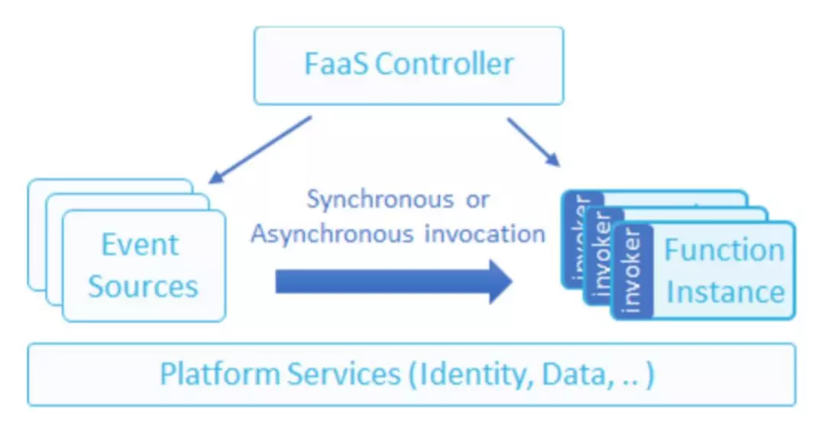
\includegraphics[width=0.7\textwidth]{Slika 7.png}
  \caption{Procesni model FaaS\newline[preuzeto sa sajta https://www.alibabacloud.com]}
  \label{fig:faasProcesniModel}
\end{figure}


Procesni model funkcije kao servis se sastoji od kontorlera funkcija (engl. Function controller), izvor događaja (engl. Event sources), instanci funkcija (engl. Function instances). Na slici se može videti procesni model FaaS\ref{fig:faasProcesniModel}. Kontroler funkcija upravlja instancama funkcija, kontroliše skaliranje instanci i izvor događaja. Izvor događaja okida funkciju iz instanci funkcija na neki događaj, npr na HTTP poziv. Funkcije dalje mogu da se izvršavaju sinhrono i asinhrono. U slučaju asinhronog izvršavanja platforma će vratiti identifikator koji se može koristi za kasniju proveru stanja funkcije \cite{sah}. Prilikom dizajniranja funkcija potrebno je pratiti princip minimalne odgovornosti (engl. single responsibility principle), što označava da funkcija treba da ima jedan zadatak koji obavlja. Funkcije je potrebno dizajnirati da budu idempotentne, što znači da višestruki pozivi iste funkcije daju iste rezultate. Da bi se obezbedila redudantnost i visoka dostupnost, funkcija može biti pozvana više od jednog puta \cite{sah}.

\section{Prednosti računarstva bez servera}

Skalabilnosti i pouzdanost računarstva bez servera koji treba da se održava. Nije potrebno praviti komplikovane distribuirane sisteme koji bi ispunili ciljeve skalabilnosti i pouzdanosti. Upravljanje pratećom infrastrukturom, njeno širenje i održavanje spada pod odgovornost pružaoca usluga.

Model plaćanja po utrošku. Tradicionalni serveri se naplaćuju bez obzira da li ima dolaznog saobraćaja. U slučaju da očekujemo povećan dolazni saobraćaj, potrebno je skalirati server unapred. To sve uvodi dodatne troškove. Modeli računarstva bez servera su granularniji po pitanju naplate. Pružalac usluga naplaćuje samo vreme koje je bilo potrebno da se funkcije izvrše. Treba imati na umu da ovaj model nije isplativiji od tradicionalnog u svim slučajevima \cite{sa}. Potrebno je postaviti prognozu inteziteta i učestalosti dolaznog saobraćaja.

Brzo isporučivanje koda na produkciono okruženje. Vreme isporučivanja rešenja do produkcije je smanjeno kako je omogućeno korisćenje postojećih servisa i resursa. Nije potrebno postavljati infrastrukturu i u BaaS modelu je moguće korišćenje nekog od postojećih rešenja.

\section{Mane računarstva bez servera}

Bojazan premeštanja podataka u javni oblak. Računarstvo bez servera predstavlja težnju da se više odgovornosti prebaci na stranu pružaoca usluga. Postoje slučajevi kada je potrebno da infrastruktura i podaci ostanu u centru podataka klijenta. U tom slučaju ne može se koristiti arhitektura bez servera\cite{sa}.

Potreba da se infrastruktura uredi na poseban način i da se sa njom upravlja. Na primer, AWS omogućava samo konfigurisanje količine ram memorije koja će biti dostupna funkciji i pruža mogućnost da se konfigurišu vrednosti tajmauta (engl. timeout). % kako prevesti timeout?

Servis mora da zadovolji nivo performansi i dostupnosti. Pružaoci usluga garantuju da će usluga biti dostupna u određenom procentu, ukoliko to nije dovoljno potrebno je dizajnirati posebno rešenje koje će zadovoljiti taj nivo. Takođe pruzaoci usluga ne garantuju nivo performansi pa je to potrebno izračunati\cite{sa}.

Zaključavanje kod pružaoca usluga (engl. vendor-locking). Ukoliko postoji potreba da arhitektura ostane nezavisna od pružaoca usluga (engl. cloud agnostic). Postoji mogućnost da se vremenom razvije jaka zavisnost od ostalih servisa koje pružalac usluga pruža. Potrebno je razmotriti koje sve servise sistem treba da koristi.
 

\section{Primeri upotrebe računarstva bez servera}

Ahritektura bez servera se može primeniti prilikom izrade kompletnog sistema, izolovanih komponenti ili pojedinačnih servisa. Prednosti računarstva bez servera je moguće iskoristiti prilikom izrade kako malih tako i velikih sistema \cite{sa}. U nastavnku su predstavljeni primeri upotrebe računarstva bez servera kod AWS pružaoca usluga.

\subsection{Servis komponenta sistema}

Tehnologije poput AWS Lambda servisa mogu da se koriste kako bi napravili zadnji kraj (engl. backend) komponentu ili servis sistema. Za primer se može uzeti servis kompanije A Cloud Guru. A Cloud Guru je platforma za učenje tehnologija oblaka čiji korisnici objavljuju snimke video lekcija. Dodatni primeri se mogu naći kod kompanija poput Comcast, Coinbase, Fender, Nordstrom i Netflix \cite{ascs}.

\subsection{IoT Tehnologije}

Arhitektura bez servera se može koristiti za implementaciju IoT (engl. Internet of Things) rešenja. AWS omogućava stvaranje IoT platforme pružanjem usluga poput, autentifikacije i autorizacije, prolaza (engl. gateway) za komunikaciju, registra za podatke o uređajima, mehanizma za čuvanje stanja uređaja, mehanizma za transformisanje poruka od uređaja ka AWS servisima \cite{aicf}. Amazon IoT platforma omogućava kreiranje servisa za uređaje bez potrebe da se održava prateća infrastruktura.

\subsection{Obrada podataka}
Može se koristiti za obradu, konverziju, manipulaciju podataka. Neki od primera su obrada CSV, JSON i XML datoteka, promena formata, obrada slika. Može se konfigurisati sistem da reaguje na događaje poput prijema slike, zatim sistem izvršava promenu formata slike u adekvatan format.

\subsection{Analiza podataka uživo}
Upliv (engl. ingestion) velike količine podataka poput podataka iz dnevnika (engl. log), transakcija, sistemskih događaja i aktivnosti korisnika može se obaviti servisima poput Amazon Kinesis Data Streams i Amazon Kinesis Firehose. Kao što se može videti na slici\ref{fig:AnalizaPodataka}, AWS Lambda servis se može koristiti da obradi podatke pre nego što se oni proslede servisima za skladištenje podataka poput S3 i Amazon DynamoDb.

\begin{figure}[!ht]
  \centering
  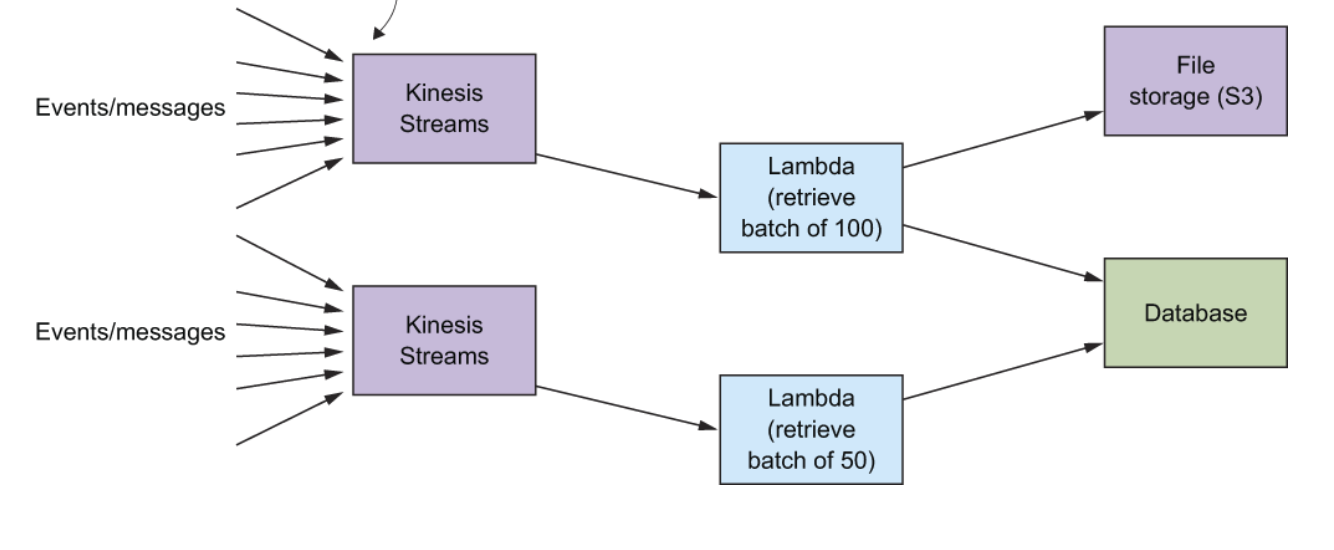
\includegraphics[width=0.9\textwidth]{Slika 8.png}
  \caption{Primer upotrebe AWS Lambda servisa za analizu podataka uživo\newline[preuzeto iz knjige Serverless architectures on AWS, autora Peter Sbarski, Yan Cui i Ajay Nair]}
  \label{fig:AnalizaPodataka}
\end{figure}

\subsection{Posrednik ka starom interfejsu} % Kako ovo prevesti Legacy API proxy

Programeri mogu da koriste Amazonove servise poput Amazon API Gateway servisa i Amazon Lambda servisa kako bi napravili međusloj između koji može da vrši obradu zahteva i njihovu konverziju u format koji je čitljiv za servise iza AWS Lambda servisa. Ovaj pristup omogućava da moderne aplikacija koriste starije servise koji koriste zastarele protokole i formate podataka. Na slici\ref{fig:KonverzijaPodataka} se može videti primer takve arhitekture.

\begin{figure}[!ht]
  \centering
  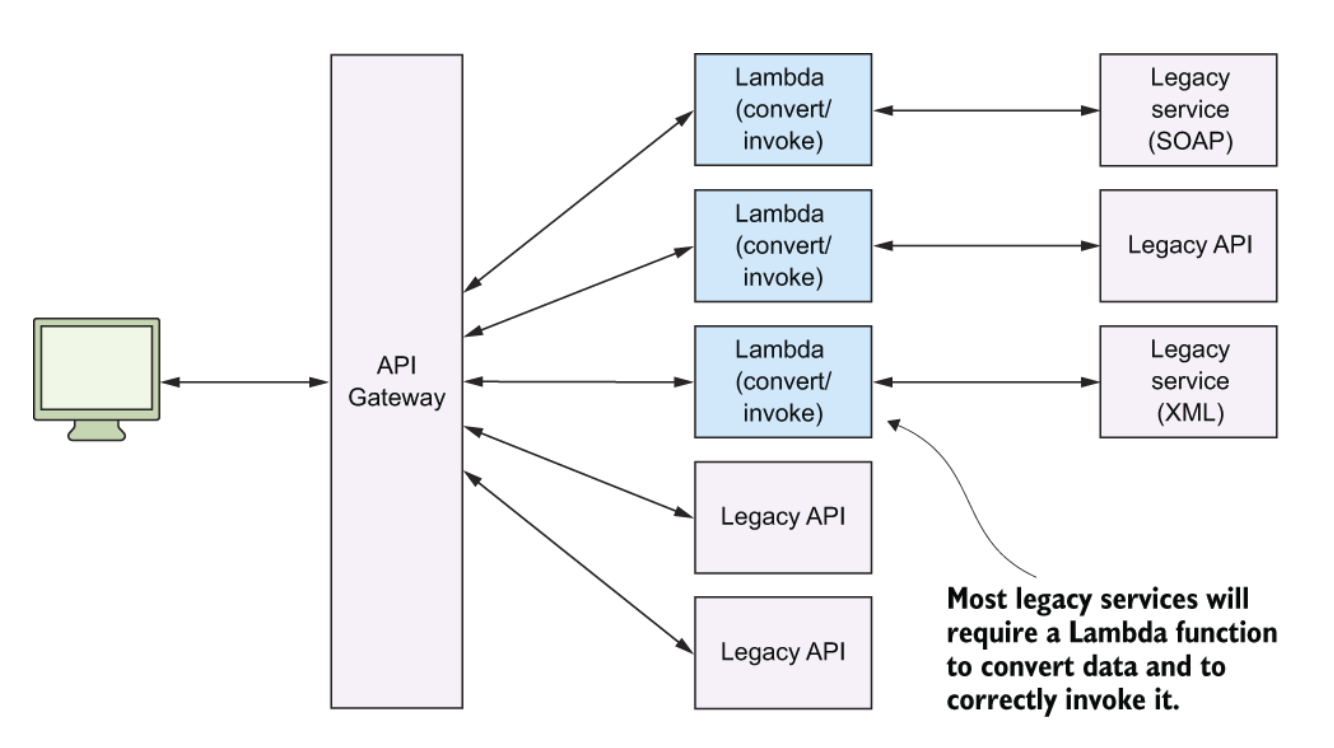
\includegraphics[width=0.7\textwidth]{Slika 9.png}
  \caption{Primer upotrebe AWS Lambda servisa za konverziju zahteva prema starijim servisima\newline[preuzeto iz knjige Serverless architectures on AWS, autora Peter Sbarski, Yan Cui i Ajay Nair]}
  \label{fig:KonverzijaPodataka}
\end{figure}

\subsection{Zakazani servisi}
%scheduled? Bolji previod?

AWS Lambda funkcije se mogu podesiti tako da rade na određenom intervalu. Te funkcije mogu izvršavati poslove pravljenja kopije podataka, uvoženje i izvoženje podataka, pravljenje podsetnika. Na primer može se konfigurisati funkcija koja će redovno kontaktirati sajt i u slučaju sa sajt nije dostupan može se poslati upozorenje na neki kanal komunikacije.

\subsection{Bot servisi}

Jedno od popularnih rešenja za primenu računarstva bez servera su bot servisi ili botovi. Botovi su aplikacije ili skripte koje rade proste poslove za neke servise, na primer za Slack. Slack bot može da reaguje na komande koje mu zada korisnik kroz aplikaciju, da vrši obaveštavanje, sakupljanje izveštaja. 

\subsection{Hibridna rešenja}

Hibridna rešenja predstavljaju kombinaciju nekog od predloženih rešenja i postojećeg sistema. Postojeći sistem se proširuje da sadrži komponente koje su razvijene arhitekturom bez servera i kao takve upotpunjuju funkcionalnosti postojećeg sistema. Na slici\ref{fig:HibridnoResenje} može se videti jedan primer takvog hibridnog rešenja koje je prošireno sa Lambda funkcijama koje obavljaju neke poslove koji nisu bili deo sistema.

\begin{figure}[!ht]
  \centering
  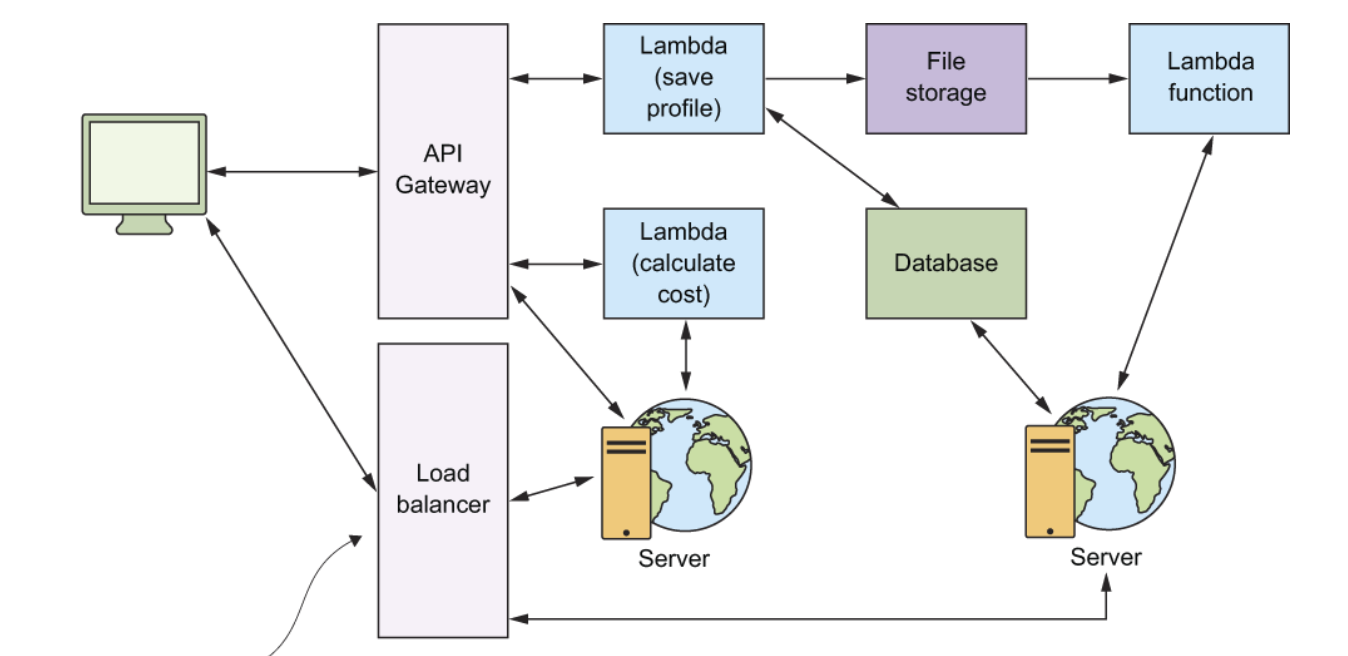
\includegraphics[width=0.7\textwidth]{Slika 10.png}
  \caption{Primer upotrebe AWS Lambda servisa za kreiranje hibridnog rešenja\newline[preuzeto iz knjige Serverless architectures on AWS, autora Peter Sbarski, Yan Cui i Ajay Nair]}
  \label{fig:HibridnoResenje}
\end{figure}

\section{Projektni uzorci}

Projektni uzorci (engl. patterns) predstavljaju rešenja za neke česte problema u dizajnu softvera. Oni takođe olakšavaju komunikaciju između programera (engl. developers) softvera ukoliko su svi upoznati sa projektnim uzorkom, njegovim prednostima i manama. Uzorci predstavljeni u ovom delu su incijalno bili korišćeni za distribuirane sisteme. Kasnije sa razvojem arhitekture bez servera ovi uzorci su postali korisni za rešavanje problema prilikom dizajniranja softvera arhitekture bez servera\cite{sa}. U nastavnku se prikazani neki od popularnih projektnih uzoraka za računarstvo bez servera.


\subsection{Komanda}
Komanda projektni uzorak enkapsulira zahtev kao objekat što omogućuje parametrizaciju klijenta različitim zahtevima, nizovima poruka i omogućava realizaciju operacija nad kojima je moguće izvršiti operaciju vraćanja na prethodno stanje (engl. undo operation) \cite{cdp}. Ovaj projektni uzorak nam omogućava da odvojimo pozivaoca operacije od servisa koji izvršava potrebnu operaciju. U praksi se ovaj projektni uzorak koristi da bi se pojednostavio interfejs i da bi se verzionisanje olakšalo.

\begin{figure}[!ht]
  \centering
  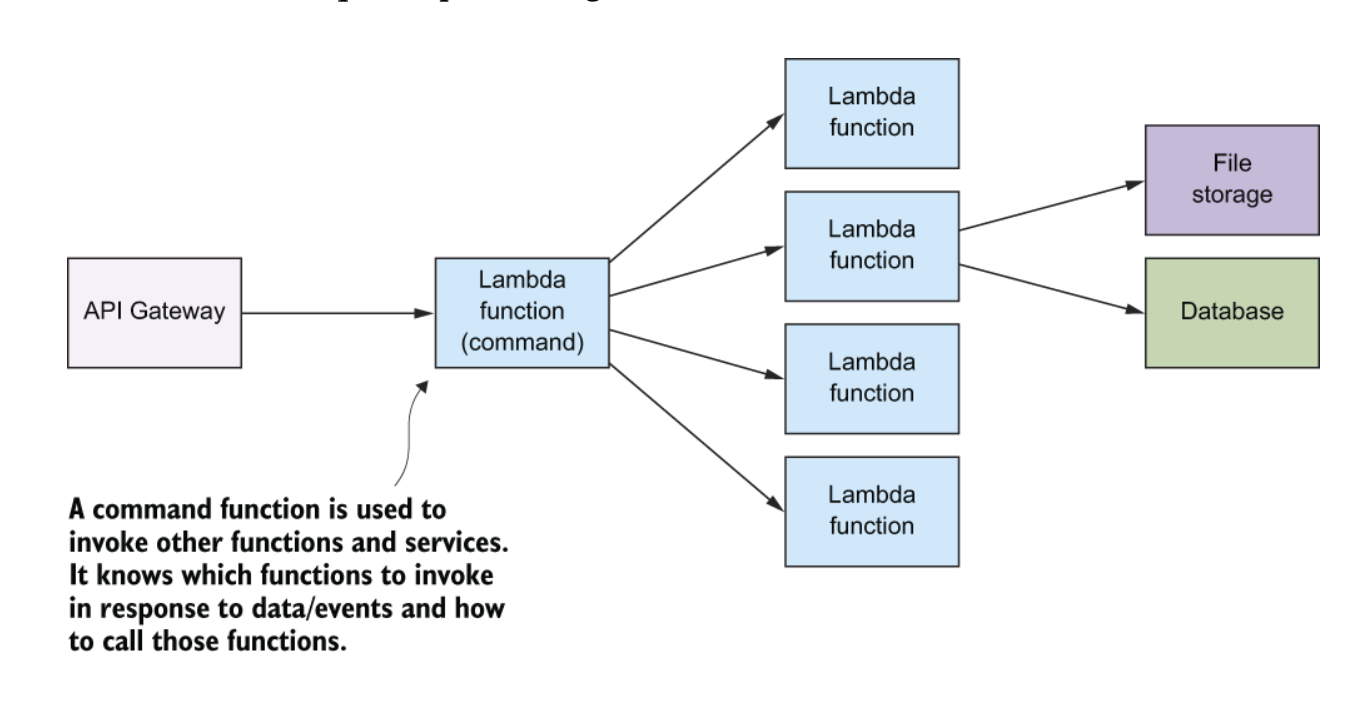
\includegraphics[width=0.8\textwidth]{Slika 12.png}
  \caption{Primer upotrebe AWS Lambda funkcije u komanda projektnom uzorku\newline[preuzeto iz knjige Serverless architectures on AWS, autora Peter Sbarski, Yan Cui i Ajay Nair]}
  \label{fig:komanda}
\end{figure}
 
Na slici\ref{fig:komanda} se može videti primer sistema koji ima posebnu AWS Lambda funkciju koja kontroliše i poziva ostale funkcije. Ona može biti prikljucena na ulaz (engl. gateway), pozvana ručno tako što joj se prosledi poruka koje funkcije da pozove. Komandna funkcija može da radi sa različitim verzijama klijenata.

\subsection{Poruke uzorak} % Kako prevesti Messaging pattern?

Poruke (engl. messaging) projektni uzorak omogućava programerima da naprave skalabilan i robusan sistem tako što se uklanjaju zavisnosti funkcija i servisa kao i skladištenje zahteva ili događaja u niz. Popularan je kod distribuiranih sistema \cite{sa}. Pouzdanost sistema poizilazi iz činjenice da servis može i da se zaustavi, sve dok su zahtevi sačuvani u nizu poruka, oni se kasnije mogu izvršiti kada se servis pokrene. Niz poruka se koristi kao bafer koji prihvata zahteve čak i kada servis koji čita iz niza ne radi. Klijent šalje zahtev koji se upisuje u niz da bi kasnije servis čitao zahteve iz samog niza. U zavisnosti kako je niz poruka konfigurisan, niz može imati više klijenata koji upisuju zahteve i više servisa koji čitaju zahteve iz niza. Na slici\ref{fig:poruke} se može videti primer impelmentacije uzorka.

\begin{figure}[!ht]
  \centering
  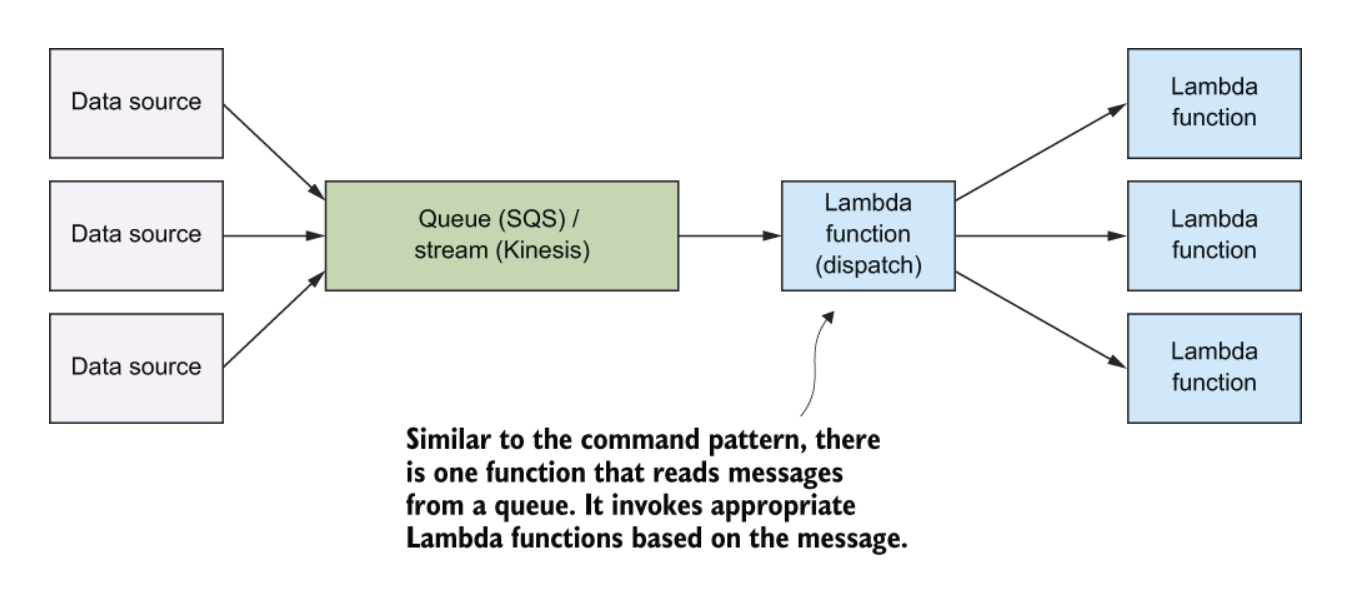
\includegraphics[width=0.8\textwidth]{Slika 13.png}
  \caption{Primer upotrebe AWS Lambda funkcije u projektnom uzorku sa porukama\newline[preuzeto iz knjige Serverless architectures on AWS, autora Peter Sbarski, Yan Cui i Ajay Nair]}
  \label{fig:poruke}
\end{figure}
 
\subsection{Nizovi sa prioritetom}
Nizovi sa prioritetom su projektni obrazac koji se koristi ukoliko postoji potreba za različitim nivoi kontole ili prioriteta. Uvođenjem dodatnih nizova postiže se da različiti nizovi mogu da se obrađuju na različrite načine. Uvođenjem prioritetnih nizova postiže se da neki zahtevi mogu da se obrade pre drugih sa manjim prioritetom. Na slici\ref{fig:nizovi} može se videti primer arhitekture sa više nizova sa različitim prioritetima.

\begin{figure}[!ht]
  \centering
  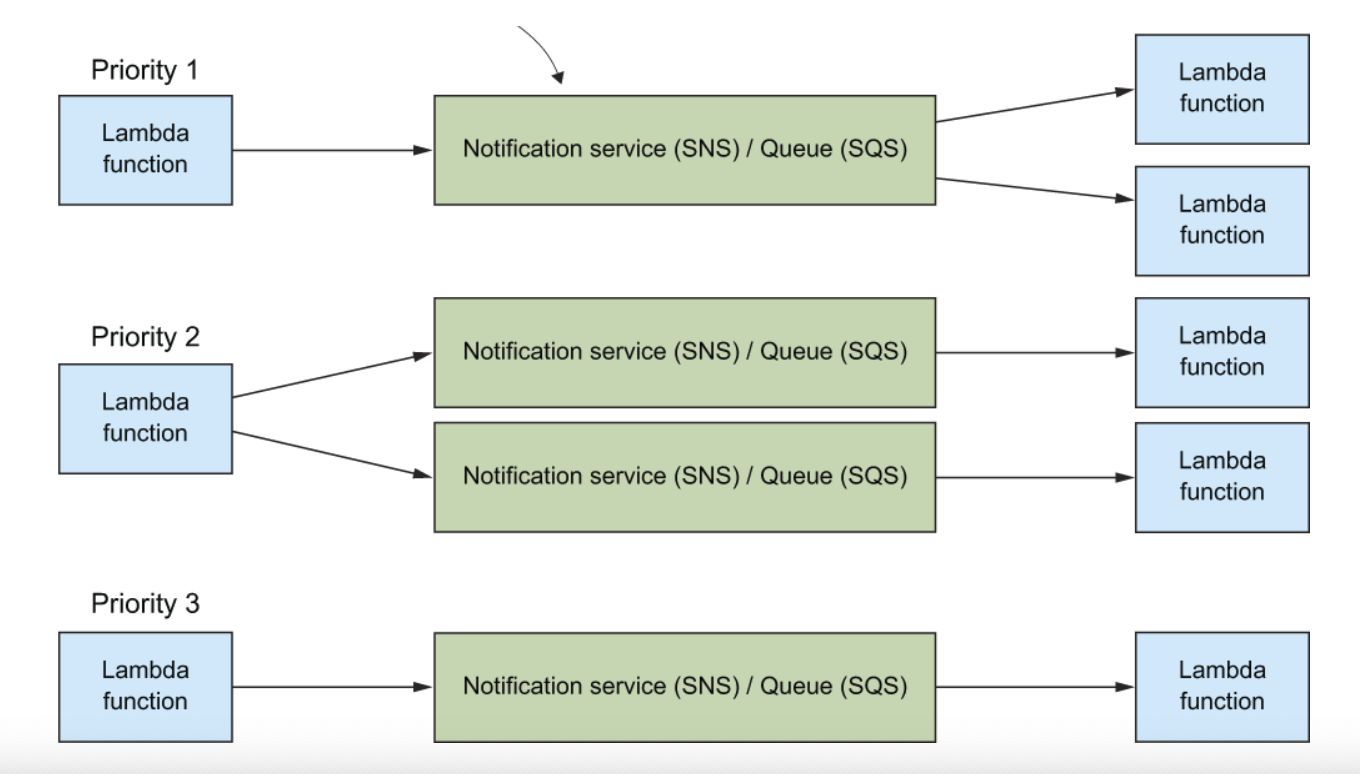
\includegraphics[width=0.8\textwidth]{Slika 14.png}
  \caption{Primer upotrebe AWS Lambda funkcije u projektnom uzorku sa prioritetnim nizovima\newline[preuzeto iz knjige Serverless architectures on AWS, autora Peter Sbarski, Yan Cui i Ajay Nair]}
  \label{fig:nizovi}
\end{figure}
 
\subsection{Grananje uzorak} % Kako ovo prevesti, fan-out?
Grananje (engl.fan-out) projektni uzorak se koristi da prosleđivanje obaveštenja i poruka svim klijentima koji slušaju ili su prijavljeni na niz za obaveštavanje (engl. messaging queue). Na AWS platformi ovaj uzorak se implementira tako što se koristi AWS SNS (engl. Simple Notification Service) tema (engl. topic) koja omogućava da se više korisnika obavesti kada se nova poruka objavi na datu temu. Još jedan primer sa AWS platforme, kada se novi fajl doda na AWS S3 servis, može se aktivirati Lambda funkcija. Za slučaj da je potrebno pozvati više funkcija, originalna AWS Lambda funkcija se može modifikovati tako da ona izvrši pozive ka odgovarajućim Lambda funkcijama, kao što je slučaj kod komanda projektnog uzorka. Ipak to zahteva više posla pa se preporučuje da se koristi AWS SNS servis koji bi pozivao funkcija u paraleli, kao što može da se vidi na slici\ref{fig:grananje}. AWS SNS teme predstavljaju komunikacione kanale koje mogu imati više izvora poruka (engl publishers) i više primalaca (engl. subscribers) koji mogu biti AWS Lambda funkcije. Kada je nova poruka objavi, AWS SNS poziva sve AWS Lambda funkcije u paraleli.

\begin{figure}[!ht]
  \centering
  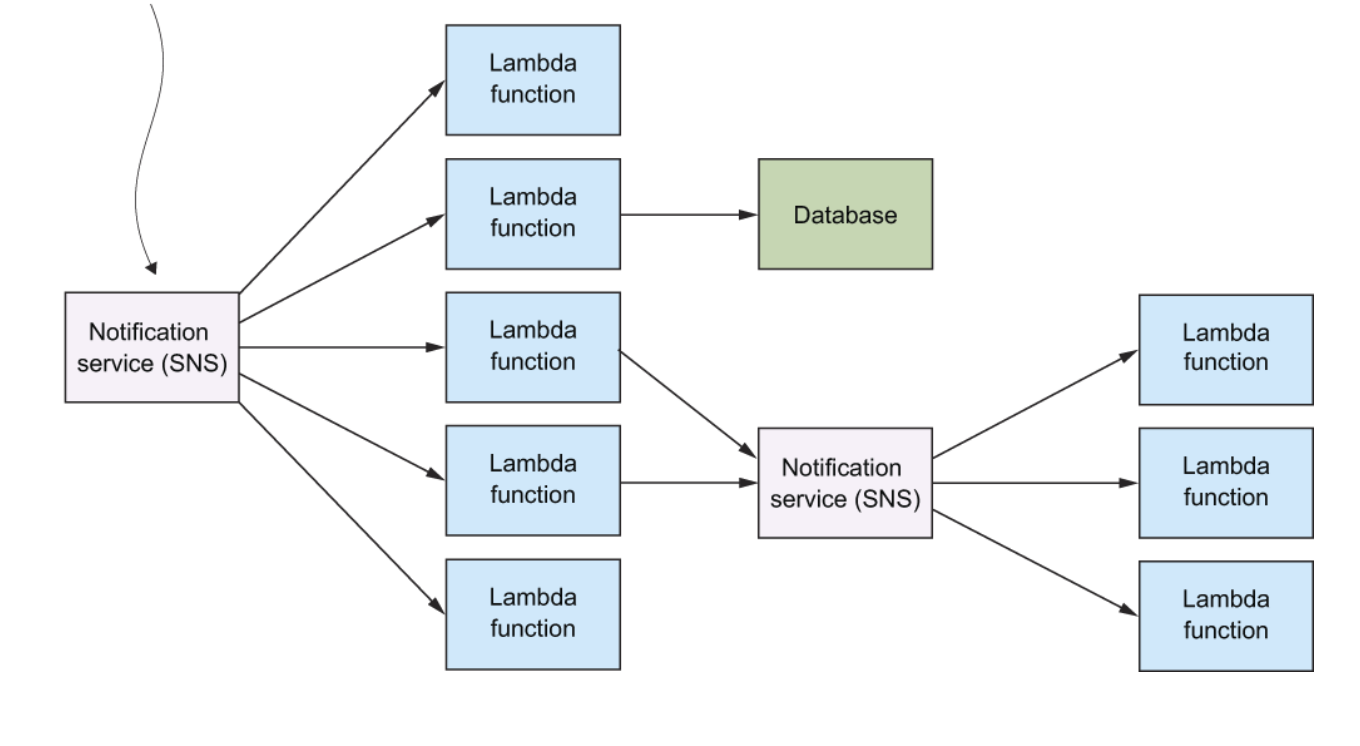
\includegraphics[width=0.8\textwidth]{Slika 15.png}
  \caption{Primer upotrebe AWS Lambda funkcije u projektnom uzorku grananje\newline[preuzeto iz knjige Serverless architectures on AWS, autora Peter Sbarski, Yan Cui i Ajay Nair]}
  \label{fig:grananje}
\end{figure}

\subsection{Računarstvo kao lepak} % Da li je dobar prevod, compute as glue?
Računarstvo kao lepak (engl. compute as glue) je projektni uzorak koji pokazuje kako Lambda funkcije mogu da se koriste za povezivanje kompleksnijih sistema. Lambda funkcije se koriste na način da one izvršavaju orkestraciju, koordinaciju i upravljanje operacijama i na taj način poput lepka vežu različite servise. U ovom stilu arhitekture, na razvijaocu je da smisli dizajn, koordinaciju i protok podataka (engl. data flow). 
 
\subsection{Tokovi i filteri uzorak}
% Kako prevesti pipeline?
Cilj ovog projektnog uzorka je razbijanje kompleksnih procesa u niz manjih servisa organizovanih u proces obrade (engl.pipeline). Komponente koje su dizajnirane da transformišu podatke se nazivaju filteri (engl. filters). Konektori koji prosleđuju podatke od jedne komponente do druge se nazivaju tokovi (engl. pipes). Preporučljivo je da svaka Lambda funkcija bude granularan servis sa jednim zaduženjem. Funkcija treba da ima jasan ulaz i izlaz sa jednostavnim interfejsom. To omogućava bolju iskorišćenost Lambda funkcija kako je one mogu koristiti u više slučajeva. Na slici\ref{fig:grananje} se može videti primer upotrebe AWS lambda funkcija.

% treba li mi ova slika?
\footnote{Slika je preuzeta iz knjige Serverless Architectures on AWS}\ref{fig:pipeline}
\begin{figure}[!ht]
  \centering
  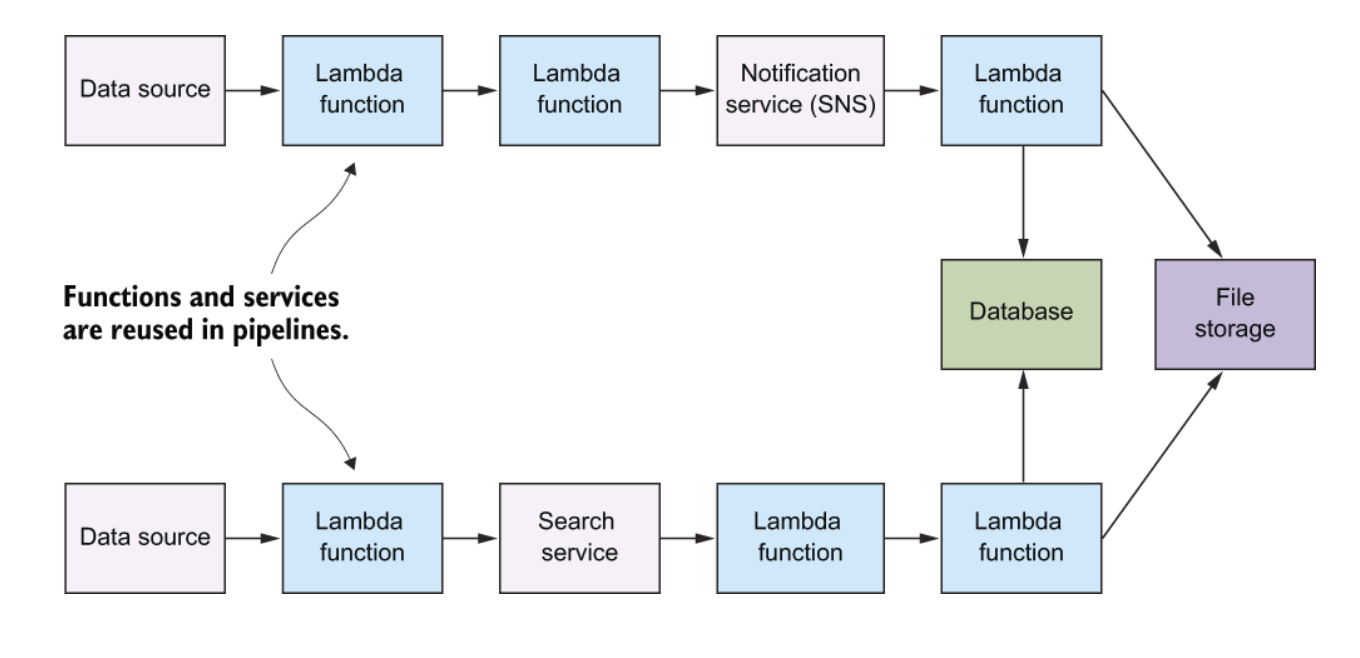
\includegraphics[width=0.8\textwidth]{Slika 16.png}
  \caption{Primer upotrebe AWS Lambda funkcije prilikom izrade kompleksnih sistema za obradu podataka\newline[preuzeto iz knjige Serverless architectures on AWS, autora Peter Sbarski, Yan Cui i Ajay Nair]}
  \label{fig:pipeline}
\end{figure}


\section{Infrastruktura kao kôd}
Kako arhitektura bez servera podrazumeva postojanje više nezavisnih funkcija za kreiranje svi potrebnih resursa koriste alati koji omogućavaju da se infrastruktura definiše kao kôd. Infrastruktura kao kôd je princip automatizovanja infrastrukture prema praksama razvijanja softvera \cite{iac}. Oslanja se na konzistentne mehanizme za kreiranje infrastrukture kao i za promenu sistema i njegovih konfiguracija. Korisnik napravi promene u svom kodu infrastrukture, zatim se oslanja na alate da provere i primene te promene na postojećem sistemu. Korišćenjem principa infrastruktura kao kod, umanjuje se trud i rizici prilikom promene na postojećoj infrastrukturi. Omogućava se korisnicima infrastrukture da dobiju resurse koje žele, kad god žele. Kreiraju se sistemi koji u zaštićeni, pouzdani. Neki od primera alata su Ansible, Chef, CloudFormation, Serverless, Puppet i Terraform. Definisanjem cele infrastrukture u formi koda, postižemo sledeće \cite{iac}:
% kako navesti alate?
\begin{enumerate}
  \item Konzistentnost. Koliko god instanci se kreira, sve će biti kreirane na isti način.
  \item Transparentnost. Svi mogu da vide šta se kreira tako što pogledaju u kôd.
  \item Ponovna iskorišćenost. Može se kreirati više instanci iste infrastrukture.
\end{enumerate}
 
\subsection{Serverles radni okvir}
 
Serverles (engl. Serverless) je radni okvir koji omogućava razvoj, isporuku koda (engl. deployment) aplikacija zasnovanih na arhitekturi bez servera. On se sastoji od interfejsa komandne linije (engl. Command-line interface - CLI) i hostovane instrument table. Zajedno olakšavaju upravljanje aplikaciom bez servera. U početku je podržavao samo AWS, da bi zatim razvio podršku i za Microsoft Azure, Google Cloud Platform, Apache OpenWhisk, Cloudflare Workers. U nastavku razmatramo primenu kod AWS pružaoca usluga. Glavni koncepti serverles radnog okvira su funkcije, događaji, resursi, servisi. 
 
Kod aplikacije zasnovane na arhitekturi bez servera je isporučen i izvršava se na AWS Lambda funkcijama. Svaka funkcija je nezavisna celina, koja se izvršava nezavisno od ostalih funkcija. Svaka funkcija treba da ima samo jedno zaduženje. Sve funkcije moraju biti definisane u serverless.yml fajlu u sekciji \emph{functions}. Prilikom definisanja funkcije potrebno je definisati njen naziv parametrom \emph{name} i kog rukovodioca funkcija koristi parametrom \emph{handler}. Rukovodilac funkcije je zapravo deo koda koji se poziva kada se pozove funkcija. Pored toga postoje i opcioni parametri koji se mogu definisati. Može se zadati opis funkcije parametrom \emph{description}, zatim može se zadati u kom okruženju se funkcija izvršava parametrom \emph{runtime}. Ne postoji mogućnost zadavanja jačine procesorske snage već se zadaje memorija koja se stavlja na raspolaganje funkciji. Memorija se zadaje u megabajtima ili MB i podrazumevana veličina je 1024. Što više memorije funkcija ima, ima i više procesorske snage. Ukoliko funkcija treba da interaguje sa nekim drugim servisom, npr sa bazom podataka, mora posedovati odgovarajuću IAM ulogu (engl. role). Uloga se zadaje pod parametrom \emph{provider.iam.role.statements} i razlikuje se u zavisnosti kom servisu za bazu podataka treba da pristupa. Moguće je jos konfigurisati oznake (engl. tags), podešavanja virtuelnog privatnog oblaka, verzionisanja, podešavanja autorizacije i tako dalje.


\begin{center}Primer definisanja funkcije u serverles radnom okviru\end{center}
\begin{lstlisting}
list:
  handler: functions/bikes/list.listBikes
  events:
    - http:
        path: bikes/list/all/location/\{location\}
        method: get
        cors: true
        authorizer:
          type: COGNITO_USER_POOLS
          authorizerId:
            Ref: ApiGatewayAuthorizer
\end{lstlisting}
 
Događaji su objekti zbog koji se pokreće funkcija. Svaka funkcija ima precizno zadatu listu događaja zbog kojih će biti pokrenuta. Ukoliko gledamo AWS pružaoca usluga, događaj može biti okačen novi fajl na S3 servisu, nova SNS tema (engl. topic), HTTP zahtev koji dolazi od aplikativnog ulaza (engl. API gateway). Nakon što se izvrši isporuka koda, radni okvir će kreirati infrastrukturu koja je potrebna da bi se napravio zadati događaj. Na primer funkcija reaguje na HTTP događaj ali nigde se ne kreira eksplicitno API Gateway. Radni okvir to prepoznaje i sam kreira API Gateway i povezuje ga sa zadatom funkciom. Funkcion radnog okvira \emph{Fn::Ref} može se referencirati na resurs koji tek treba da bude kreiran.
 
Servisi predstavljaju organizacione jedinice u serverles radnom okviru. Servis je konfigurisan u serverless.yml fajlu gde su definisane i funkcije, događaji koji ih okidaju kao i ostali resursi koji se koriste. Kako aplikacija raste, preporučljivo je da se formira više servisa u skladu sa funkcionalnostima \cite{sfs}. Od verzije 3.15.0, moguće je korišćenje više servisa, paralelno i sekvencijalno isporučivanje koda (engl. deployment). Uveden je i novi fajl serverless-compose.yml u kome se nalaze konfiguracije kompozitnih servisa.
 
Resursi predstavljaju sve infrastrukturne resurse koji su neophodni funkcijama. Na primer ukoliko funkcija čuva rezultat u bazi podataka, onda je on definisana kao resurs. Resursi se definišu parametrom \emph{resources} i u slučaju AWS pruzaoca usluga, koristi se sintaksa CloudFormation šablona (engl. template).


\chapter{Veb servis na arhitekturi bez servera za iznajmljivanje bicikala}
 
U ovom poglavlju je predstavljena implementacija servisa zasnovanog na arhitekturi bez servera i na AWS Lambda platformi. U prvom delu poglavlja je predstavljena arhitektura servisa, zatim je objašnjen proces kreiranja resursa u oblaku i isporučivanja koda. U poslednjem delu poglavlja se prolazi kroz korišćene AWS servise. Servis je isporučen i javno dostupan na AWS platformi korišćenjem pogodnosti besplatnog (engl. free-tier) naloga. Servis je razvijen kao projekat otvorenog koda i celokupan je javno dostupan na adresi https://github.com/Vojkan-Cvijovic/Rent-A-Bike. Za razvoj servisa korišćen je programski jezik JavaScript i radni okvir Node.js 14. Za razvojno okruženje je korišćen WebStorm koji je razvijen od strane JetBrains kompanije.


\section{Arhitektura servisa}

Veb servis je zamiljen kao zadnji deo (engl. backend) aplikacije za iznajmljivanje bicikala. Korisnik preko aplikacije može da odabere i rezerviše biciklu dok servis treba da omogući izvršavanje zadatih operacija i čuvanje rezultata tih operacija. Za razvoj servisa je odabrana arhitektura bez servera kako se sistem sastoji od više jednostavnih operacija koje mogu predstavljati funkcije sistema i kako se očekuje promenljiv intenzitet dolaznog saobraćaja. Očekuje se da dolazni zahtevi pristižu servisu samo u određenim delovima dana kao naprimer ujutru ili uveče dok tokom noći neće dolaziti ni jedan zahtev. Arhitektura bez servera najbolje zadovoljava zahteve prikazanog veb servisa.

Servis omogućava korisnicima dohvatanje lokacija gde se bicikle nalaze zatim kreiranje, brisanje, dohvatanje svih bicikli, dohvatanje samo slobodnih bicikli, ažuriranje bicikli. Funkcionalnosti servisa se ostvaruju preko pojedinačnih funkcija. Svaka funkcija ima samo jedno zaduženje. Na primer funkcija za kreiranje bicikli, prihvata podatke poput proizvođača, godine proizvodnje, lokacije i vraća odgovor o uspešnosti izvršenja operacije. Funkcije su isporučene AWS Lambda servisu i za svaku funkciju je napravljen jedna Lambda funkcija. U podešavanjima funkcija je navedena na koji tip događaja se funkcija aktivira i koji rukovodilac se koristi. Sve funkcije se aktiviraju na neki oblik HTTP zahteva koji dolazi sa aplikativnog ulaza (engl. gateway). Kod HTTP zahteva razlikujemo putanju, promenljive iz putanje, tip zahteva. Rukovodioci (engl. handlers) funkcija su moduli koji su napisani u JavaScript programskom jeziku, svaki modul pripada samo jednoj funkciji. Servisu se pristupa preko aplikativnog ulaza. Za autentifikaciju i autorizaciju se koristi servis AWS Cognito. Kako AWS Lambda funkcije ne čuvaju stanje, sve promene na sistemu se upisuju u bazu podataka. Za bazu podataka servis koristi servis pod nazivom AWS DynamoDB, koji nam omogućava da koristimo no-sql bazu podataka. Za upis u bazu podataka funkcije koriste \emph{aws-sdk}  biblioteku koja ima implementaciju klijenta za pristup bazi u okviru modula \emph{AWS.DynamoDB}. Dnevnik o funkcionisanju (engl. log) čuva servis pod nazivom AWS CloudWatch koji nam omogućava grupisanje podataka po funkcijama i pretragu za zadato vreme. Na slici\ref{fig:awsArchitecture} se može videti skica AWS arhitekture servisa.

\begin{figure}[!ht]
  \centering
  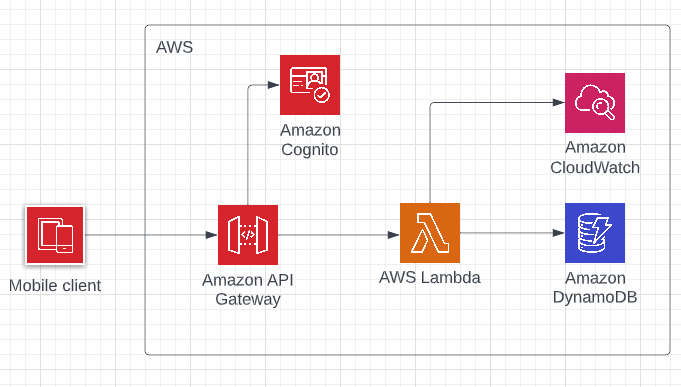
\includegraphics[width=0.7\textwidth]{AWS-Architecture-Overview.PNG}
  \caption{Prikaz arhitekture servisa zajedno sa svim AWS servisima koji su deo servisa}
  \label{fig:awsArchitecture}
\end{figure}


\subsection{Struktura projekta}
Servis je podeljen po direktorijumima po funkcionalnosti. U nastavku su opisani direktorijumi, njihovo značenje kao i datoteke koje se u njima nalaze.

\begin{enumerate}
  \item Konfiguracije eksternih servisa koje koristimo iz funkcija se nalaze u direktorijumu \emph{config}. U našem slučaju servis direktno koristi samo bazu podataka tako da config folder sadrži samo jedan fajl dynamoDB.js gde je napravljen klijent za bazu podataka koji se posle koristi u svakoj funkciji.
  \item \emph{functions/bikes}. Sadrži sve funkcije na projektu. Svaka funkcija ima svoj JavaScript fajl i zadružena je samo za jednu funkcionalnost. 
  \item \emph{onboarding}. Sadrži instrukcije za podešavanje lokalnog okruženja za rad sa servisom.
  \item \emph{serverless}. Sadrži instrukcije za serverles (engl. serverless) radni okvir koji je zadužen za kreiranje i azuriranje AWS resursa. Konfiguracije su sadržane u YAML fajlovima i grupisane su po zaduženjima. Direktorijum sadrži konfiguracioni fajl za bazu podataka, autentifikaciju, autorizaciju i za funkcije.
  \item \emph{utils}. Direktorijum sa funkcionalnostima koje trebaju da se dele. Na primer servis uvek vraća JSON odgovor pa je u common.js fajlu definisan mehanizam za kreiranje JSON odgovora kao i za postavljanje odgovarajućih zaglavlja koja se uvek vraćaju.
  \item \emph{.gitignore}. Za verzionisanje servisa se koristi alat pod nazivom Git. Ovaj fajl nam omogućava da naznačimo koje fajlove želimo da git ignoriše.
  \item \emph{serverless.yml}. Glavni fajl koji serverles radni okvir čita. U njemu su sadržane reference ka ostalim fajlovima iz serverless direktorijuma.
\end{enumerate}

\subsection{Funkcije}
U ovom poglavlju su definisane sve funkcije koje su razvijene kao deo servisa. Sve funkcije se aktiviraju na odgovarajući HTTP zahtev sa aplikativnog ulaza i proizvode odgovor u JSON formatu. U tabeli \ref{tbl:funkcije} su opisane sve funkcije servisa. Za svaku funkciju je naveden koji metod i koju putanju treba da se napravi HTTP poziv da bi se željena funkcija aktivirala.

\begin{table}
  \centering
  \caption{Opis funkcija servisa}
  \label{tbl:funkcije}
  \begin{tabular}{|p{2cm}|p{7cm}|p{4cm}|} % dimenzije?
    \hline
      Metod& Putanja & Opis \\
    \hline
    GET & bikes/list/all/location/\{location\} & Vraća niz svih bicikli koje su kreirane na zadatoj lokaciji.\\
    \hline
    GET & bikes/list/available/location/\{location\} & Vraća niz dostupnih bicikli na zadatoj lokaciji.\\
    \hline
    GET & bikes/list/locations & Vraća niz lokacija na kojima ima kreiranih bicikli.\\
    \hline
    POST & bikes/create & Kreira biciklu sa prosleđenim vrednostima.\\
    \hline
    GET & bikes/\{id\} & Vraća informacije za biciklu sa zadatim identifikatorom.\\
    \hline
    PATCH & bikes/update/used & Označavanje da li je bicikla iznajmljena ili je završeno iznajmljivanje.\\
    \hline
    PATCH & bikes/update/active & Deaktiviranje i aktiviranje bicikli. \\
    \hline
    DELETE & bikes/delete/\{id\} & Briše biciklu iz baze podataka.\\
    \hline
  \end{tabular}
\end{table}

U nastavku rada je prikazana implementacija funkcije za kreiranje bicikli. Funkcija prima proizvođača bicikle, godinu proizvodnje, lokaciju na kojoj će bicikla biti dodata kao i status bicikle. Funkcija koristi \emph{uuid} biblioteku za generisanje identifikatora bicikle. U zavisnosti od uspešnosti operacije, funkcija vraća odgovarajuću poruku korisniku.

\begin{center}Primer implementacije funkcije za kreiranje bicikala\end{center}
\begin{lstlisting}
module.exports.createBike = async event => {
  const body = JSON.parse(event.body);
  const id = uuid.v1();
  try {
      const { manufacturer, year, location, active } = body;
      const used = false
      const TableName = process.env.BIKES_TABLE_NAME;
      const params = {
          TableName,
          Item: {
              id,
              manufacturer,
              year,
              location,
              active,
              used
          },
          ConditionExpression: "attribute_not_exists(id)"
      };
      await dynamoDb.put(params).promise();
      return sendResponse(200, { message: 'Bike created successfully with id ' + id });
  } catch (e) {
      console.log(e);
      return sendResponse(500, { message: 'Could not create the bike with id ' + id });
  }
};
\end{lstlisting}

\section{Korišćeni AWS servisi}
\subsection{Lambda}
 
AWS Lambda je servis koji ne čuva stanje (engl. stateless) i pokreće se događajima (engl. event-driven) koji omogućava pokretanje aplikacije bez kreiranja i održavanja servisa. Lambda pokreće zadati kôd na računarskoj infrastrukturi velike dostupnosti (engl. high-availability) i stara se o administraciji računarskih resursa. Održavanje servera, operativnog sistema, kapaciteta za proširivanje, automatskog proširivanja (engl. automatic scaling) spada pod nadležnosti AWS Lambda servisa. Na korisniku je da prosledi Lambda servisu kôd napisan u jednom od podržanih jezika. U trenutku pisanja ovog rada, Lambda podržava Node.js, Python, Ruby, Java, Go, .NET razvojna okuženja \cite{lr}.
 
Lambda servis omogućava organizovanje koda po Lambda funkcijama. Lambda pokreće funkciju u zavisnosti od podešavanja funkcije i stara se o horizontalnom skaliranju. Korisnik plaća samo vreme izvršavanja funkcija. Lambda ne dozvoljava korisnicima da se uloguju na instancu ili da naprave posebne izmene na operativnom sistemu. Korisniku se omogućava da zada veličinu memorije koja se stavlja na raspolaganje funkciji. Veličina memorije je povezana za jačinom procesorske snage i količinom mrežnog protoka.
 
Isporučivanje (engl. deployment) koda Lambda funkciji se vrši preko paketa isporučivanja (engl. deployment package). Lambda podržava dva paketa za isporučivanje:
\begin{enumerate}
  \item Kompresovana \emph{.zip} arhiva. Ona mora da sadrži ceo kôd kao i sve zavisnosti koje kôd ima. Lambda funkcija obezbeđuje operativni sistem i okruženje u kome kôd radi.
  \item Slika kontejnera (engl. container image). Slika mora da bude kompatibilna sa specifikaciom OCI (engl. Open Container Initiative). Ona mora da sadrži kôd, sve zavisnosti, operativni sistem i okruženje u kome će kôd biti pokrenut.
\end{enumerate}
 
Lambda automatski pokreće dodatne instance funkcije u slučaju da je funkcija pozvana pre nego sto je tekuća funkcija završila. Kada se protok saobraćaja smanji, Lambda servis zaustavlja ili uklanja trenutne instance. Plaća se samo vreme koje je bilo potrebno funkciji da se inicijalizuje i da obradi zahtev. Lambda servis ima dva limita skaliranja, limit konkurentnosti i limit naletne konkuretnosti (engl. burst concurrency). Oba limita se ne primenjuju na konkretnu Lambda funkciju već obuhvataju sve Lambda funkcije u regionu korisnika. Limit konkurentnosti je od 1000, dok je limit naletne konkuretnosti od 500 i oba zavise od regiona. Posle inicijalnog naleta zahteva, nakon što imamo 500 funkcija da rade paralelno, broj novih paralelnih funkcija se može povećati za 500 po minutu i nastavlja dok ne dostigne limit konkurentnosti. Prema tome kao što se može videti na slici \ref{fig:awsLambdaSkaliranje}, Lambda servis nam garantuje određenu količinu instanci čiji broj se uvećava ekponencijalno dok posle tog limita, broj instanci funkcija raste linearno. Ukoliko zahtevi dolaze brže nego sto broj funkcija može da raste ili je maksimalan broj funkcija iskorišćen, ti zahtevi će pasti sa status kodom 429. Za slučaj da se kôd na funkcijama sporo inicijalizuje, Lambda servis podržava konfigurisanje broja funkcija koje će uvek biti dostupne. Time ste postiže da imamo određenu količinu funkcija koje mogu odmah da odgovore na zahteve.
 

\begin{figure}[!ht]
  \centering
  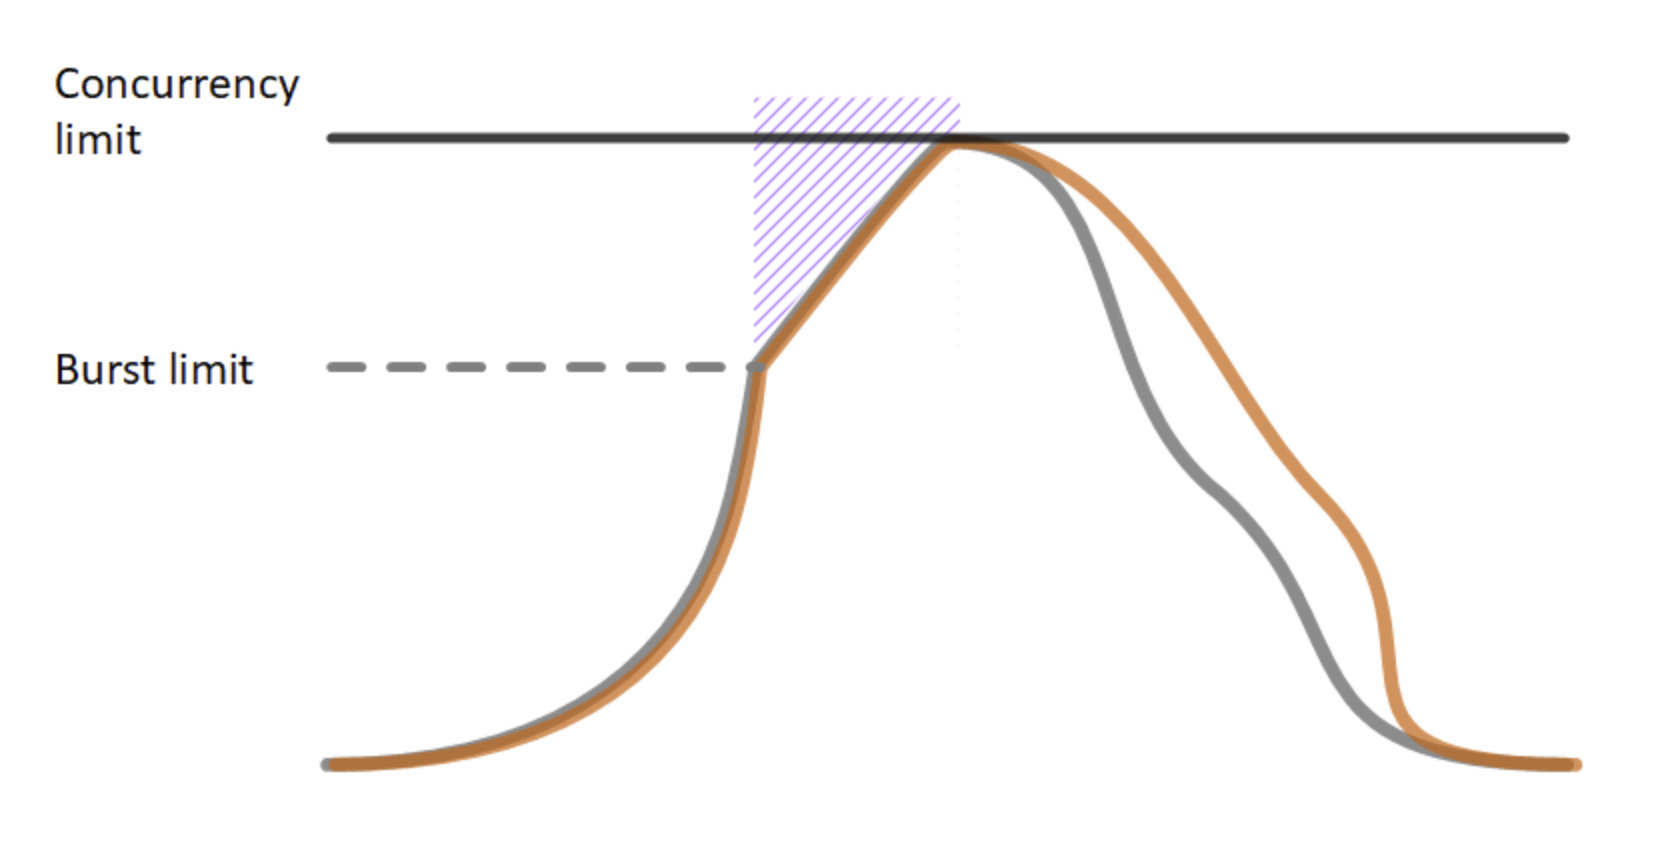
\includegraphics[width=0.7\textwidth]{AWS-Lambda-skaliranje.png}
  \caption{Grafikon skaliranja Lambda funkcija\newline[preuzeto sa sajta https://docs.aws.amazon.com/lambda/latest/dg/invocation-scaling.html]}
  \label{fig:awsLambdaSkaliranje}
\end{figure}
 
Lambda servis podržava podelu koda u biblioteke. Lambda sloj (engl. layer) omogućava da arhiva, koja je isporučuje Lambda funkciji, ima dodatni kôd ili neki drugi sadržaj. Lambda sloj omogućava da se sve zavisnosti pakuju u biblioteke čime se postiže bolja iskorišćenost koda. Redukuje veličinu arhive koju je potrebno proslediti funkciji, samim tim se i vreme slanja arhive smanjuje pa se i kôd brže isporučuje. Funkcije koje koriste sliku kontejnera ne mogu da koriste Lambda slojeve već one moraju da imaju sve upakovano u sliku kontejnera.

 
Da bi se kontrolisala prava pristupa funkcije ostalim AWS servisima, svakoj Lambda funkciji je dodeljena posebna IAM uloga (engl. role) za izvršavanje. Ovoj ulozi je moguće dodati polisu koja definiše prava pristupa određenim AWS servisima i resursima. Ukoliko Lambda funkcija poziva druge servise iz koda putem AWS biblioteke, potrebno je proširiti ovu polisu da bi omogućili funkciji da izvrši zahtev. Preporučljivo je pratiti princip minimalnog pristupa prilikom izrade polisa, što znači Lambda funkciji dozvoliti da izvršava samo servise koji su joj neophodni. 

 
Lambda servis pokreće funkcije u bezbednom i izolovanom okruženju za izršavanje (engl. execution environment). Okruženje upravlja resursima potrebnim za izvršavanje i životnim ciklusom (engl. lifecycle) okruženja za izršavanje funkcije. Životni ciklus okruženja se deli na faze inicijalizacije (engl. Init), pozivanja (engl. invoke) i zaustavljanja (engl. shutdown) što se može videti na slici \ref{fig:awsLambdaZivotniVek}. U fazi inicijalizacije, Lambda servis kreira ili startuje okruženje sa konfigurisanim resursima, pribavlja kôd za funkciju i sve Lambda slojeve (engl. layers), inicijalizuje ekstenzije i radni okvir, zatim poziva kôd za incijalizaciju funkcije. Ovaj redosled osigurava da je radno okruženje spremno za izvršavanje koda funkcije. U fazi izvršavanja, Lambda servis poziva rukovodioca funkcije koji je postavljen kada je funkcija napravljena. Nakon što se završi izvršavanje funkcije, Lambda servis zamrzava okruženje funkcije. Faza zaustavljanja se poziva ukoliko Lambda funkcija nije pozivana određeno vreme. U ovoj fazi Lambda servis zaustavlja radno okruženje, obaveštava sve ekstenzije da se zaustavlja i na kraju uklanja radno okruženje. Kod Lambda funkcije razlikujemo takozvani hladni start (engl. cold start) i topli start (engl. warm start). Kod hladnog starta ne postoji okruženje za izvršavanje pa Lambda izvršava sve korake incijalizacije okruženja zatim se startuje funkcija. Dok kod toplog starta, već postoji okruženje ali je ono zamrznuto pa se izvršava samo inicijalizacija funkcije i zatim startovanje funkcije. Pojava hladnog starta uvodi dodatno kasnjenje u sistem. 
 

\begin{figure}[!ht]
  \centering
  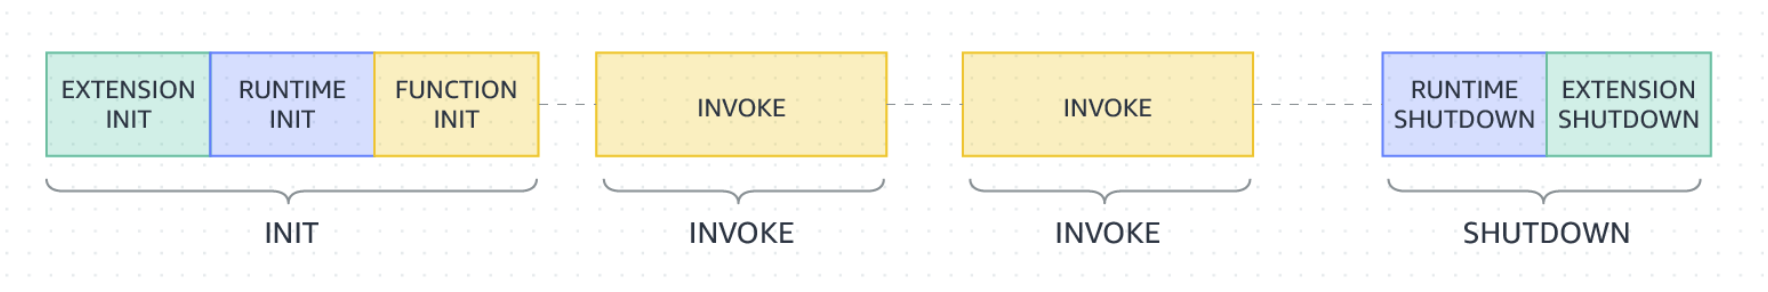
\includegraphics[width=0.9\textwidth]{AWS-Lambda-zivotnivek.png}
  \caption{Životni vek Lambda funkcije\newline[preuzeto sa sajta https://docs.aws.amazon.com/lambda/latest/dg/lambda-runtime-environment.html]}
  \label{fig:awsLambdaZivotniVek}
\end{figure}
 
% monitoring and operation tools -> kako prevesti?
Lambda ekstenzije omogućavaju proširivanje okruženja za izvršavanje koda Lambda funkcija. Preko ekstenzija klijenti mogu da itegrišu svoje alate bez potrebe instalacije i upravljanja konfiguracijama. Ekstenzije mogu biti uključene kao Lambda sloj ili kao deo slike kontejnera. Neki od primera alata koji se koriste u ekstenzijama su HashiCorp Vault za skladištenje osetljivih podataka, NewRelic za praćenje performansi sistema, Splunk za vođenje dnevnika.

\subsection{API Gateway}
 
Amazon API ulaz (engl. gateway) je servis koji omogućava kornisnicima da kreiraju, isporučuju, održavaju i obezbede aplikativni programsi interfejs. On predstavlja ulaz za klijentske aplikacije do servisa. Korišćenjem ovog servisa moguće je kreirati aplikativne programske interfejse zasnovane na REST stilu ili zasnovane na veb soketima koji omogućavaju dvosmernu komunikaciju između aplikacija. REST API se koristi za slučajeve jednosmerne komunikacije, klijent je taj koji inicira komunikaciju i potržuje podatke od servera. Kod veb soketa potrebna je dvosmerna komunikacija, server ima potrebu da obavesti klijenta, na primer server kod aplikacija za dopisivanje. API ulaz omogućava upravljanje konkurentnim pozivima, autorizaciom, kontrolom pristupa, ograničavanjem broja poziva (engl. throttling), praćenjem (engl. monitoring) i upravljanjem verzija interfejsa. Za autorizaciju API ulaz može da koristi pristup zasnovan na IAM polisama ili posebnu AWS Lambda funkciju koja će verifikovati posebne JWT (engl. JSON Web Token) tokene ili SAML zahteve. Amazon ne naplaćuje kreiranje ulaz već se naplata vrši prema broju zahteva koje API ulaz primi kao i prema količini podataka koju prenese. 
 
\subsection{CloudFormation}
 
AWS CloudFormation je servis koji omogućava modelovanje i kreiranje AWS resursa čime se uprošćava upravljanje infrastrukturom. Servis omogućava korisniku da kreira novi ili modifikuje postojeći CloudFormation šablon (engl. template). Za slučaj da postoji potreba da servis bude dostupan u dodatnim regionima potrebno je replicirati sve resurse iz postojećeg regiona. U slučaju otkaza, korisnici mogu da koriste infrastrukturu iz drugog regiona. CloudFormation servis olakšava replikaciju infrastrukture po regionima korišćenjem šablona. Resursi i servisi se definišu jednom a mogu se koristiti proizvoljan broj puta. Servis olakšava kontolu i prećenje promena na infrastrukturi. Kako je šablon zapravo tekstualni fajl, mogu se pratiti sve promene koje se dešavaju sa tekstualnim fajlom putem sistema za verzionisanje.
 
CloudFormation servis radi sa dva resursa, šablonom (engl. template) i stekom (engl. stack). Šablon se koristi da bi se opisali AWS resursi i njihove funkcionalnosti. Šablon može biti JSON ili YAML struktuirani tekstualni fajl. Stek je organizaciona jedinica CloudFormation servisa. Prilikom kreiranja, ažuriranja ili brisanja steka resursi se kreiraju, ažuriraju ili brišu. Svi resursi u steku su definisani u odgovarajućem CloudFormation šablonskom fajlu.
 
\subsection{IAM}
 
IAM je servis za autentifikaciju i autorizaciju na AWS platformi. Omogućav da kreiranje korisnika i da im se dodele mogućnost da izvrše određene operacije. Podržava i mogućnost podešavanja višestruke autentifikacije (engl. multi-factor authentication - MFA). Ukoliko je uključen MFA, korisnici moraju pored šifre ili pristupnog (engl. access) ključa da proslede još i kôd sa specijalno konfigurisanog uređaja ili aplikacije. IAM servis funkcioniše po modelu eventualne konzistentnosti. Zbog potrebe visokog nivoa dostupnosti, servis vrši replikaciju podataka preko servera u Amazonovim centrima podataka, pa je potrebno vremena da se promene propagiraju kroz sistem. U nastavku navodimo resurse IAM servisa:
\begin{enumerate}
  \item Korisnik (engl. user). Predstavlja osobu ili servis koji interaguje sa AWS servisima. Pruža mogućnost autentifikacije korisnika ili servisa.
  \item Korisnička grupa (engl. user groups). Kolekcija korisnika koja olakšava upravljanje permisijama korsnika.
  \item Uloge (engl. roles). Može biti dodeljena korisniku ili grupi i služi da naznači sta je korisniku dozvoljeno da izvrši.
  \item Polise (engl. policies). Predstavljaju JSON dokument koji je pridružen ulozi, korisniku, grupi korisnika ili nekom AWS resursu i služi da definiše permisije.
\end{enumerate}

\subsection{Cognito}
 
Amazon Cognito pruža usluge autentifikacije i autorizacije. Korisnik može da napravi korisnika i da se uloguje sa njim ili može da se uloguje preko drugih servisa kao na primer Facebook, Amazon, Google ili Apple. Dve glavne komponente servica su grupe korisnika (engl. user pool) i grupe identiteta (engl. identity pool). Grupe korisnika su korisnički direktorijumi koji omogućavaju da se korisnik registruje i prijavi. Omogućavaju i prijavu preko eksternih servisa. Podržava i napredne bezbednosne mehanizme poput višestruke autentifikacije (engl. multi-factor authentication) kao i verifikaciju telefona, mail naloga. Grupe identiteta omogućavaju da korisnik dobije privremene AWS kredencijale sa kojima je moguć pristup AWS servisima poput AWS S3 ili AWS DynamoDB. Podržavaju jos i pristup anonimnih korisnika ukoliko postoji potreba da im se dodele određeni resursi.

% TODO Kako prevesti user pool? identities pool?

\begin{figure}[!ht]
  \centering
  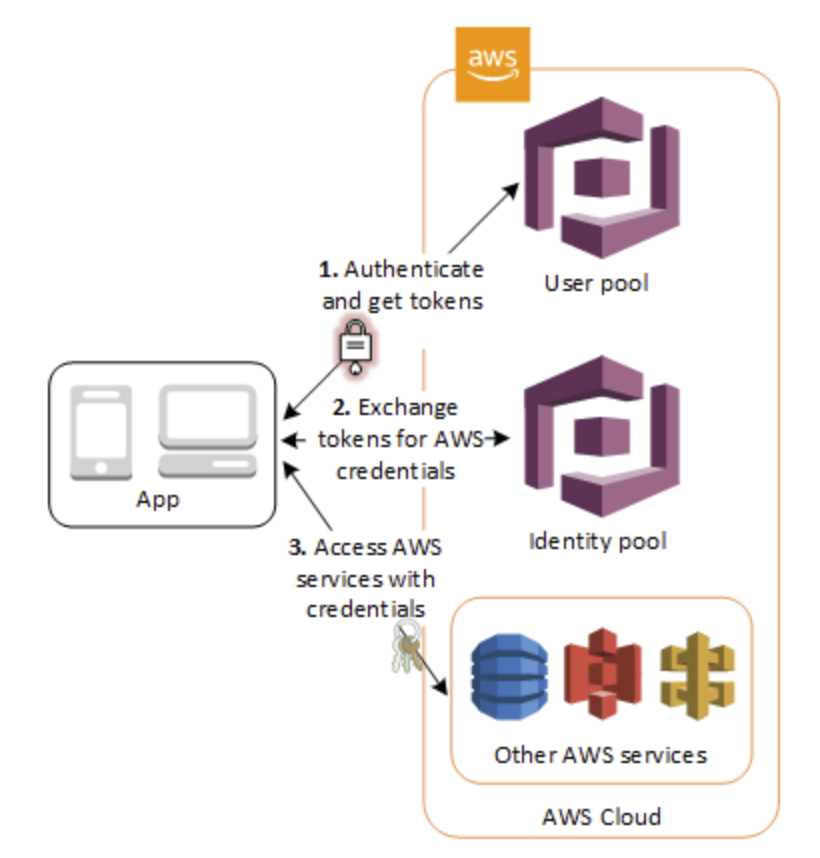
\includegraphics[width=0.5\textwidth]{ProcesAutentifikacije.png}
  \caption{Proces autentifikacije kada se koriste grupe korisnika i grupe identiteta\newline[preuzeto sa sajta https://docs.aws.amazon.com/cognito/latest/developerguide/what-is-amazon-cognito.html]}
  \label{fig:procesAutentifikacije}
\end{figure}

% da li da se navodi u listi?
Kao što se može videti na slici \ref{fig:procesAutentifikacije}, proces autentifikacije se može podeliti na 3 koraka:
\begin{enumerate}
  \item Korisnik se uloguje sa kredencijalima na grupu korisnika, u slučaju uspešne autentifikacije u odgovoru dobija tokene.
  \item Korisnik prosleđuje tokene koje je dobio u prvom koraku i za uzvrat dobija privremene AWS kredencijale.
  \item Poslednji korak je da korisnik uz pomoć dobijenih kredencijala pravi poziv ka odabranom AWS servisu kao na primer AWS S3.
\end{enumerate}

\subsection{DynamoDB}

Amazon DynamoDB je servis koji pruža skalabilnu NoSql bazu podataka. Amazon je zadužen za upravljanje i skaliranje distribuirane baze te korisnik ne mora da se stara o konfigurisanju i replikaciji sadržaja. Servis omogućava enkripciju podataka u bazi tako da to nije potrebno odraditi u servisima koji upisuju u bazu. Korisniku je omogućeno da kreira tabele i da čuva proizvoljnu količinu podataka kao i da ima proizvoljan broj zahteva ka bazi. DynamoDB omogućava pravljenje rezervnih kopija na zahtev kao mogućnost oporavka na osnovu rezervne kopije. Takođe servis omogućava povratak na bilo koji trenutak u poslednjih 35 dana čime se baza čuva od slučajnih operacija pisanja ili brisanja. Rekordima u bazi je moguće i postaviti vreme koje se čuvaju (engl. time to live - TTL) čime se redukuje prostor potreban za skladištenje podataka a samim tim i troškovi korišćenja servisa smanjuju. DynamoDB automatski raspoređuje podatke i dolazni saobraćaj na potreban broj servera. Svi podaci se čuvaju na SSD (engl. solid-state) diskovima i automatski se repliciraju po zonama u regionu. Ukoliko konfigurišemo tabelu da bude globalna, servis će replicirati podatke po svim AWS regionima.

\chapter{Mobilna aplikacija za iznajmljivanje bicikala}
 
U cilju demonstracije upotrebe tehnologija opisanih u prethodnim glavama, razvijena je android aplikacija koja omogućava korisniku da odabirom lokacije vrši pretragu bicikli. Korisnik dalje može da rentira biciklu pa ga zatim aplikacija preusmerava na sledeću stranicu gde ima pregled koliko dugo je bicikla iznajmljena. Kada korisnik završi sa iznajmljivanjem, bicikla se vraća u listu bicikli koje mogu da se iznajme. Da bi korisnik koristio aplikaciju mora da poseduje nalog koji može da napravi kroz aplikaciju. Ukoliko korisnik ima admin privilegije, omogućava mu se da kroz aplikaciju kreira i briše nove bicikle i lokacije. Korisnik može postati admin tako što se doda u admin grupu na AWS Cognito servisu.
 
Aplikacija je napisana u Kotlin programskom jeziku i koristi Retrofit biblioteku za apstrakciju API poziva ka veb servisu. Prvo je predstavljen Kotlin programski jezik i pokazano je zašto je on odabran umesto Jave. Zatim se prolazi kroz Retrofit biblioteku koju aplikacija koristi. U poslednjem delu se prolazi kroz samu aplikaciju, arhitekturu aplikacije i bitnije delove koda aplikacije.
\section{Kotlin}
Kotlin je jedan od novijih programskih jezika kreiran od strane kompanije JetBrains. Ime je dobio po ostrvu Kotlin u blizini Sankt Petersburga. Razvoj je započet 2010 godine, prva verzija je bila dostupna javnosti 2012. Prva stabila verzija pod nazivom 1.0 je uvedena 2016 godine. Važan trenutak u istorijatu Kotlina se dogodio 2017. godine kada je na Google I/O konferenciji, Google Android tim zvanično podržao Kotlin kao prvi izbor za razvoj aplikacija na Android platformi. 
 
 
Po definiciji Kotlin je statički tipiziran programski jezik za razvoj multiplatformskih aplikacija. Kotlin je koncizan, interoperabilan, bezbedan, sa odličnim razvojnim alatima i okruženjem. Nastao je sa ciljem da se prevaziđu nedostaci koje je imao programski jezik Java. Kotlin se kompajlira u bajt kôd (engl. bytecode) i pokreće na Java virtuelnoj mašini. Na ovaj način se ostavlja mogućnost kompanijama da postepeno migriraju kôd sa Jave na Kotlin. Treba naglasiti da sintaksa ovog jezika nije kompatibilna sa Java jezikom. Može se kompajlirati u JavaScript kôd ili koristiti LLVM kompajler.

 
\subsection{Koncepti}
Kotlin je slican Javi, pa je i samim tim veliki broj koncepata preuzet iz Jave. U nastavku su predstavljeni osnovni koncepti Kotlin jezika. 
\subsubsection{Struktura}
Specifikacija paketa treba da bude zadata na pocetku fajla i navodi se kljucnom rečju \emph{package}. Uključivanje dodatnih paketa se postiže na isti način kao u Javi, sa ključnom rečju \emph{import}. Kljucna rec za definiciju funkcije je \emph{fun}. Kotlin programskom jeziku mora da ima funkciju main i ona ne mora imati argumente. 
 
\begin{center} Primer 1: Struktura Kotlin dokumenta\end{center}
\begin{lstlisting}[language=Java]
package demo.app
 
import kotlin.text.*
 
fun main() {
    println("Hello from Kotlin app!")
}
\end{lstlisting}
 
\subsubsection{Promenljive}
U Kotlin programskom jeziku postoje dva tipa promenljivih a to su promenljive i konstante. Za promenljive se koristi ključna reč \emph{var} i njihova vrednost može da se promeni nakon dodele. Za konstante se koristi ključna reč \emph{val} i jednom kada dodelimo vrednost ne može se promeniti. Kotlin ne zahteva eksplicitno navođenje tipa svake promenljive i u stanju je da to zaključi u vreme kompajliranja iz izraza sa kojim vršimo dodelu vrednosti.

\begin{center} Primer 2: Promenljive\end{center}
\begin{lstlisting}[language=Java]
val constant = 2.71828
var i = 0
 
constant = 3        // Greska!
i += 1              // i = 1 
\end{lstlisting}
 
\subsubsection{Funkcije}
Funkcije u Kotlin jeziku se navode koristeći ključnu reč \emph{fun}. Parametri funkcije se definišu prateći Paskalovu notaciju, \emph{ime: tip}. Parametri se odvajaju zapetom i tip parametra mora biti naveden u potpisu funkcije. Kotlin podržava definisanje podrazumevanih vrednosti argumenata funkcije. U zavisnosti gde su definisane, u Kotlinu razlikujemo 3 tipa funkcija: globalne, lokalne i funkcije koje su član neke klase ili objekta (engl. member). Globalna funkcija je definisana van svake klase. Lokalna funkcija je funkcija koja je definisana unutar postojeće funkcije.
 
\subsubsection{Naredbe račvanja}
 
U Kotlinu ključna reč \emph{if} se koristi kao izraz izračunavanja nekog uslova. U Kotlinu ne postoji ternarni operator pošto if komanda vraća rezultat. Za razliku od jave koja ima \emph{switch} komandu, Kotlin ima \emph{when} komandu koja predstavlja naredbu višestrukog grananja.

\begin{center} Primer 3: Naredbe grananja\end{center}
\begin{lstlisting}[language=Java]
var max = x
if (x < y) max = y
 
// if with else
var max: Int
if (x > y) {
    max = x
} else {
    max = y
}
 
// if as expression
val max = if (x > y) x else y
 
// when with default 
when (x) {
    1 -> print("x == 1")
    2 -> print("x == 2")
    else -> {
        print("x is neither 1 nor 2")
    }
}
\end{lstlisting}
 
 
\subsubsection{Petlje}
Osnovne petlje u Kotlinu su \emph{for}, \emph{while} i \emph{do-while} petlje. For petlja iterira koristeći iterator i ekvivalentna je \emph{foreach} pelji u JavaScript programskom jeziku. Razlika između \emph{while} i \emph{do-while} petlje je u tome što \emph{while} petlja proverava uslov pre izvršavanja bloka dok \emph{do-while} petlja prvo izvrši blok pa tek onda proverava uslov. Kotlin podržava tradicionalne \emph{break} i \emph{continue} operatore u petljama.

\begin{center} Primer 4: Petlje u Kotlin jeziku\end{center}
\begin{lstlisting}[language=Java]
for (i in array.indices) {
    println(array[i])
}
 
var num = 4 
while (num > 0) {
  num--
}
 
do {
    val y = retrieveData()
} while (y != null)       // y je vidljivo ovde 
\end{lstlisting}
 
\subsubsection{Nula vrednosti}
Kotlin pokušava da reši problem pristupanja nula (engl. null) vrednostima. Pristup članu instance koja ima nula vrednost proizvodi \emph{NullPointerException} izuzetak u Javi. U Kotlinu, svaka promenljiva je podrazumevano ne nula vrednost. Kako bi se dozvolilo da promenljiva sadrži nula vrednost, mora se to izričito naglasiti. To se postiže dodavanjem upitnika prilikom definisanja tipa promenljive. U sledećem primeru se može videti kako izgleda upravljanje nula vrednostima u Kotlin jeziku.

\begin{center} Primer 5: Dodela nula vrednosti\end{center}
\begin{lstlisting}[language=Java]
var nonNullString: String = "abc" // Inicijalizacija ne nula vrednoscu
nonNullString = null              // Greska u fazi kompajliranja
 
var nullableStr: String? = "abc"  // String moze biti nula vrednost
nullableStr = null                // Ok
 
val l = nullableStr.length        // Greska, vrednost moze biti nula
\end{lstlisting}
 
Da bi se pristupilo vrednosti promenljive koja može biti nula, mora se ograditi naredbom grananja i proveriti vrednost. Drugi način je da se koristi operator \emph{?.} koji vraća vrednost ako promenljiva nije nula vrednost inače vraća nula vrednost. U nastavku se može videti na primeru.
 
\begin{center} Primer 6: Upravljanje nula vrednostima\end{center}
\begin{lstlisting}[language=Java]
var b: String?
val l1 = if (b != null) b.length else -1  // prvi nacin
 
var l2 = b?.length                        // drugi nacin
\end{lstlisting}
 
Kotlin je uveo i operator \emph{!!} koji izvršava proveru vrednosti promenljive. U slučaju da je vrednost nula, operator baca grešku. Operator pruža sigurnost da vrednost koja se dodeljuje promenljivoj neće imati nula vrednost.
 
\begin{center} Primer 7: Koršćenje operatora !!\end{center}
\begin{lstlisting}[language=Java]
var b: String?
val l = b!!.length
\end{lstlisting}
 
\subsubsection{Klasa}
Klase u Kotlin jeziku se deklarišu koristeći ključnu reč \emph{class}. Klasa u kotlinu može da ima primarni konstruktor i jedan ili više sekundarnih konstruktora. Primarni konstruktor je deo zaglavlja klase i navodi se posle naziva klase sa svojim agrumentima. Primarni konstruktor ne može da ima u sebi kôd već kôd koji je potreban za inicijalizaciju se upisuje u inicjalizacioni blok i to se postiže ključnom rečju \emph{init}. Prilikom inicijalizacije instance, inicjalizacioni blokovi se izvršavaju u redosledu u kome su navedeni u telu klase. Parametri primarnog konstruktora se mogu koristiti iz inicjalizacionih blokova. Oni se takođe mogu koristiti prilikom inicijalizacije polja klase. Polja klase se odvajaju zapetama. 
 
\begin{center} Primer 8: Klasa u Kotlin jeziku\end{center}
\begin{lstlisting}[language=Java]
class Person(val name: String) {
    val children: MutableList<Person> = mutableListOf()
    constructor(name: String, parent: Person) : this(name) {
        parent.children.add(this)
    }
}
\end{lstlisting}
 
Sekundarni konstruktori moraju imati prefix \emph{constructor}. Ukoliko klasa sadrži primarni konstruktor, svaki sekundarni konstruktor mora da sadrži direktan ili indirektan poziv primarnog konstruktora. To se postize ključnom rečju \emph{this} zatim se u zagradi navode argument primarnog konstruktora. Kotlin ne sadrži ključnu reč \emph{new} pa se instanciranje klase obavnja navođenjem imena klase, zatim se unutar zagrada navode argumenti. Slično kao i Java, Kotlin podržava apstraktne klase koje se ne mogu instancirati. Definišu se ključnom rečju \emph{abstract} dok se nasleđivanje vrši operatorom \emph{:}.
 
Čest primer upotrebe klase je čuvanje podataka. Iz ovog razloga nam Kotlin nudi poseban tip klase nazvan klasa podataka (engl. data class). Ispravno definisana klasa podataka mora da sadrži:
\begin{enumerate}
  \item primarni konstruktor sa barem jednim argumentom.
  \item argument primarnog konstruktora mora biti označen sa val ili var.
  \item klase podataka ne mogu biti apstrakne, otvorene, zaključane (engl. seald) ili unutrašnje.
\end{enumerate}


Za sve deklarisane argumente u primarnom konstruktoru u klasi podataka kompajler će generisati funkcije za proveru jednakosti (engl. equals()), funkciju za pristup svakom parametru \emph{componentN()} gde N predstavlja redni broj argumenta, izračunavanje heš koda (engl. hashCode()), funkciju za kopiranje (engl. copy()), funkciju za ispis polja kao nisku (engl. toString()) u specijalnom formatu. Razlog uvođenja klase podataka je smanjivanje koda koji mora da se napiše da bi se postigna neka funkcionalnost. U nastavku je prikazano definisanje klase u Javi kao i kako bi se ista ta klasa definisala u Kotlinu kao klasa podataka.

\begin{center} Primer 9: Java klasa\end{center}
\begin{lstlisting}[language=Java]
  public final class User {
    private final String name;
    private final int age;

    public String getName() {
        return this.name;
    }
    public int getAge() {
        return this.age;
    }

    @Override
    public String toString() {
        return "User{" +
                "name='" + name + '\'' +
                ", age=" + age +
                '}';
    }

    @Override
    public boolean equals(Object o) {
        if (this == o) return true;
        if (o == null || getClass() != o.getClass()) return false;
        User user = (User) o;
        return age == user.age && Objects.equals(name, user.name);
    }

    @Override
    public int hashCode() {
        return Objects.hash(name, age);
    }

    public User() {
        this.name = "";
        this.age = 0;
    }

    public User(String name) {
        this.name = name;
        this.age = 0;
    }

    public User(int age) {
        this.name = "";
        this.age = age;
    }

    public User(String name, int age) {
        this.name = name;
        this.age = age;
    }
}
\end{lstlisting}
U nastavku se može videti primer iste klase u Kotlin programskom jeziku. Funkcionalnost ostaje ista dok je sintaksa konciznija.
\begin{center} Primer 10: Kotlin klasa\end{center}
\begin{lstlisting}[language=Java]
data class User(val name: String = "", val age: Int = 0)
\end{lstlisting}

\section{Aplikacija}
U ovom poglavlju je predstavljena android aplikacija koja je razvijena u cilju ilustracije opisanih tehnologija. Android aplikacija je napisana u programskom jeziku Kotlin i zahteva barem Android 11 operativni sistem ili neki noviji. Prvo su predstavljeni arhitektura aplikacije i opis biblioteke za komunikaciju sa servisom a zatim opis upotrebe aplikacije.
 
\subsection{Arhitektura aplikacije}
 
Aplikacija je sastavljena od aktivnosti i postoji tačan redosled kojim se aktivnosti mogu pokrenuti. Inicijalna aktivnost je stranica za prijavljivanje. U zavisnosti da li korisnik postoji, aplikacija može da pređe na aktivnost za registraciju ili da pristupi prijavljivanju korisnika. Ukoliko korisnik se korisnik uspesno prijavi na aplikaciju, u zavisnosti od da li spada u administratore ili ne, korisnik se može preusmeriti na aktivnosti za izlistavanje lokacija ili na administratorsku stranicu.
 
\begin{figure}[!ht]
  \centering
  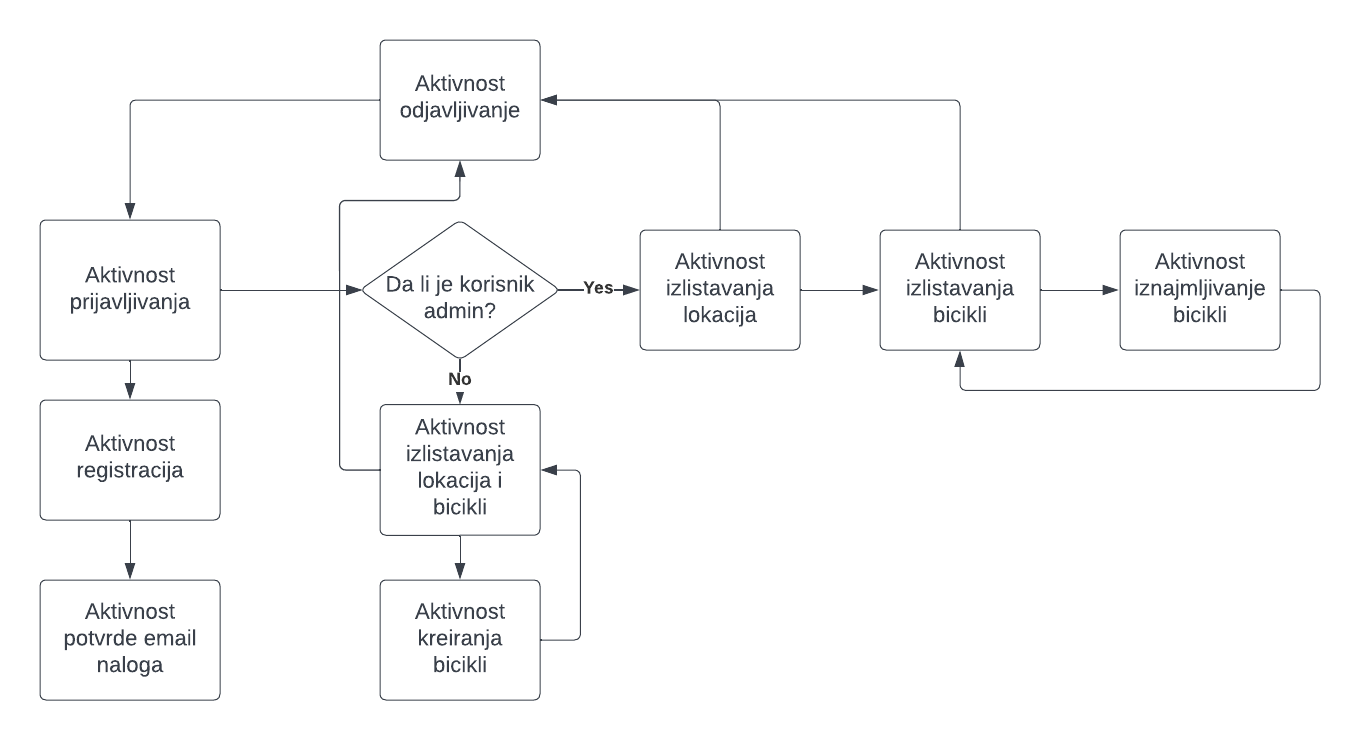
\includegraphics[width=0.8\textwidth]{Organizacija aktivnosti.png}
  \caption{Arhitektura aplikacije}
  \label{fig:arhitekturaApplikacije}
\end{figure}
 
Za regularnog korisnika, početna aktivnost je stranica koja pokazuje lokacije gde postoje bicikle za iznajmljivanje. Sa te aktivnosti korisnik može da ide na aktivnost za odjavljivanje sa aplikacije ili da produži na aktivnost za prikazivanje bicikli. U slučaju da ode na aktivnost za odjavljivanje, korisnik se odjavljuje i vraća na stranicu za prijavljivanje. Ako korisnik produži na aktivnost za prikazivanje bicikli, odatle može da ide na dve aktivnosti, za iznajmljivanje bicikli ili na aktivnost za odjavljivanje. Kada jednom ode na aktivnost za iznajmljivanje bicikli, korisniku je omogućeno samo da se vrati na aktivnost za prikazivanje bicikli, nije ponuđeno da se korisnik odjavi sa aplikacije.
 
Za admin korisnika, početna aktivnost pokazuje stranicu lokacije i u zavisnosti bicikli u zavisnosti od lokacije. Korisniku je omogućeno da promeni stanje bicikle, obriše i kreira biciklu. Brisanje i menjanje stanja bicikle su funkcionalnosti koje obavljaju u okviru iste aktivnosti dok za kreiranje bicikle postoji posebna aktivnost. Sa obe aktivnosti korisniku je omogućeno da ide na aktivnost za odjavljivanje sa aplikacije.
 
% navodnici ili ?
Sve aktivnosti su definisane u direktorijumu \emph{src/main/java/org/bikerent}. Svaka aktivnosti ima poseban Kotlin fajl i sve aktivnosti su registrovane u manifestu na putanji \emph{src/main/AndroidManifest.xml}. Izgledi korisničkog interfejsa su definisani na putanji \emph{src/main/res/layout/} i svaka aktivnost ima svoj odgovarajući XML fajl. Za autentifikaciju android aplikacija koristi biblioteku kosmos\footnote{izvorni kôd je dostupan https://github.com/jamesonwilliams/kosmos} i prilikom povezivanja aplikacije sa AWS Cognito servisom potrebno je popuniti konfiguracije u BikeRentApp na putanji \emph{src/main/java/org/bikerent/BikeRentApp.kt}.
 
\subsection{Biblioteka za komunikaciju za veb servisom}
 
Za potrebe demonstracije razvijen je javno dostupan REST servis koji se izvršava kod Amazon pružaoca usluga u regionu centralne evrope. U android aplikaciji koristimo biblioteku pod nazivom \emph{Retrofit}\footnote{izvorni kôd je dostupan https://square.github.io/retrofit/}. Retrofit je javno dostupna biblioteka koja olakšava pravljenje HTTP API poziva ka servisu. Biblioteka ima za cilj da se reši koda koji uvek mora da se napiše (engl. boilerplate code) kada se pravi API poziv. To se postiže tako što se HTTP aplikativni interfejs preslikava u interfejs u Kotlin programskom jeziku. Kao što se može videti u primeru, biblioteka se oslanja na anotacije za definisanje specifičnosti zahteva poput tela, parametara, tipa zahteva. Takođe biblioteka radi sa klasama podataka (engl. data class) čime se dodatno uprošćava korišćenje same biblioteke.

\begin{center} Primer 11: Interfejs za izvršavanje GET API poziva\end{center}
\begin{lstlisting}[language=Java]
public interface GitHubService {
  @GET("users/{user}/repos")
  Call<List<Repo>> listRepos(@Path("user") String user);
}
\end{lstlisting}


Retrofit biblioteka generiše instancu interfejsa koji je definisan u primeru iznad. Potrebno joj je proslediti putanju na kojoj se servis nalazi. Nad klijentom se dalje poziva metoda create kojoj se prosleđuje klasa od koje želimo da klijent napravi servis.
\begin{center} Primer 12: Inicijalizacija Retrofit klijenta i primer korišćenja\end{center}
\begin{lstlisting}[language=Java]
Retrofit retrofit = new Retrofit.Builder()
  .baseUrl("https://api.github.com/")
  .build();

GitHubService service = retrofit.create(GitHubService.class);
Call<List<Repo>> repos = service.listRepos("octocat");
\end{lstlisting}


Biblioteka vraća objekat tipa Call od zadatog servisa. Call objekat može napraviti sinhroni ili asinhroni zahtev ka veb serveru. Instanca Call klase se može iskoristiti samo jednom. Ukoliko je potrebno koristiti je više puta, postoji opcija poziva funkcije \emph{clone()} koja će vratiti novu instancu Call klase.
 
\subsection{Upotreba aplikacije}
 
\subsubsection{Proces registracija i prijavljivanja korisnika}
 
Kada kornisnik instalira aplikaciju od njega se zahteva da se uloguje na aplikaciju. Ukoliko korisnik nema nalog, postoji opcija da kroz aplikaciju napravi nalog. Kada odabere da napravi nalog, korisniku se otvara sledeći prozor\ref{fig:registracijaKorisnika} u kome mu se trazi da unese podatke o email adresi i šifri. Potrebno je da korisnik prosledi validnu email adresu. Aplikacija poseduje i validaciju email adrese. Takođe potrebno je da korisnik unese šifru koja će zadovoljiti sledeće uslove:

\begin{enumerate}
  \item Sadrži barem 8 karaktera.
  \item Sadrži barem jedno malo slovo.
  \item Sadrži barem jedno veliko slovo.
  \item Sadrži barem jedan specijalan karaktera.
  \item Sadrži barem jedan broj.
\end{enumerate}
 
%TODO Kako organizovati ove slike? Koja visina i sirina?
\begin{figure}[!ht]
  \centering
  
\includegraphics[height=0.6\textwidth]{Registracija.jpg}
  % 
\includegraphics[width=0.7\textwidth]{Registracija.jpg}
  \caption{Registracija korisnika}
  \label{fig:registracijaKorisnika}
\end{figure}

 
Ukoliko korisnik unese šifru ili email koji ne zadovoljavaju uslove unosa, aplikacija izbacuje tekstualnu poruku sa opisom koja je validacija pala. Na primer, korisnik unese šifru koja ima 7 karaktera, aplikacija izbacuje poruku da šifra mora da ima barem 8 karaktera. Nakon što korisnik unese validan email i validnu šifru, pritiskom na drugme za registraciju, korisnik se prebacuje na sledeći prozor. Na sledećem prozoru, aplikacija traži od korisnika verifikacioni kôd. Potrebno je da korisnik potvrdi email tako što će uneti verifikacioni kôd koji mu servis posalje na email. Ukoliko korisnik ne unese kôd, servis smatra da nalog nije verifikovan i korisnik ne može da se prijavi na aplikaciju.
 
\subsubsection{Upotreba aplikacije regularnog korisnika}
 
Kada korisnik potvrdi nalog, omogućava mu se prijavljivanje na aplikaciju. Korisnik to čini preko prozora za prijavljivanje. Potrebno je da korisnik unese email kao korisničko ime i šifru. Ukoliko korisnik ne unese jedno od obaveznih polja, aplikacija izbacuje grešku. Aplikacija takođe validira da je korisničko ime u formatu emaila. Za slučaj da korisnik unese pogrešno korisničko ime, odnosno unese za korisnika koji nije registrovan na platformi, aplikacija izbacuje poruku da zadati korisnik ne postoji. Za slučaj da korisnik unese ispravano korisničko ime a neispravanu šifru, aplikacija obaveštava korisnika da prosleđena šifra nije ispravna.
 
Kada se prijavi na aplikaciju, korisniku se pokazuje lista lokacija bicikli. Na istom prozoru postoji mogućnost da se korisnik odjavi sa aplikacije. Odabirom lokacije korisnik se prebacuje na sledeći prozor\ref{fig:odabirBicikle} gde dobija listu dostupnih bicikli. Korisnik ne može da dobije u ponudi biciklu koju je neki drugi korisnik iznajmio, već dobija samo bicikle koje on može da iznajmi. Pored bicikli korisniku je ostavljena mogućnost da se odjavi sa aplikacije. Kada jednom odabere biciklu, pritiskom na dugme, korisnik može da je iznajmi i tada prelazi na sledeći ekran. Kada iznajmi biciklu, korisniku na ekranu se pojavljuje štoperica koja služi da naznači koliko je dugo bicikla iznajmljena. Sa tog prozora korsinik može da prekine iznajmljivanje bicikle i tada se vraća na prethodni prozor gde mu aplikacija nudi spisak dostupnih bicikli za zadatu lokaciju. Jednom odabrana lokacija ostaje upamćena dok je korisnik ne promeni pa iz tog razloga korisnik se vraća na spisak bicikli za inicijalno odabranu aplikaciju. Korisnik ima mogućnost da se vrati sa prozora bicikli na prozor izabranih lokacija i da promeni lokaciju.
 

\begin{figure}[!ht]
  \centering
  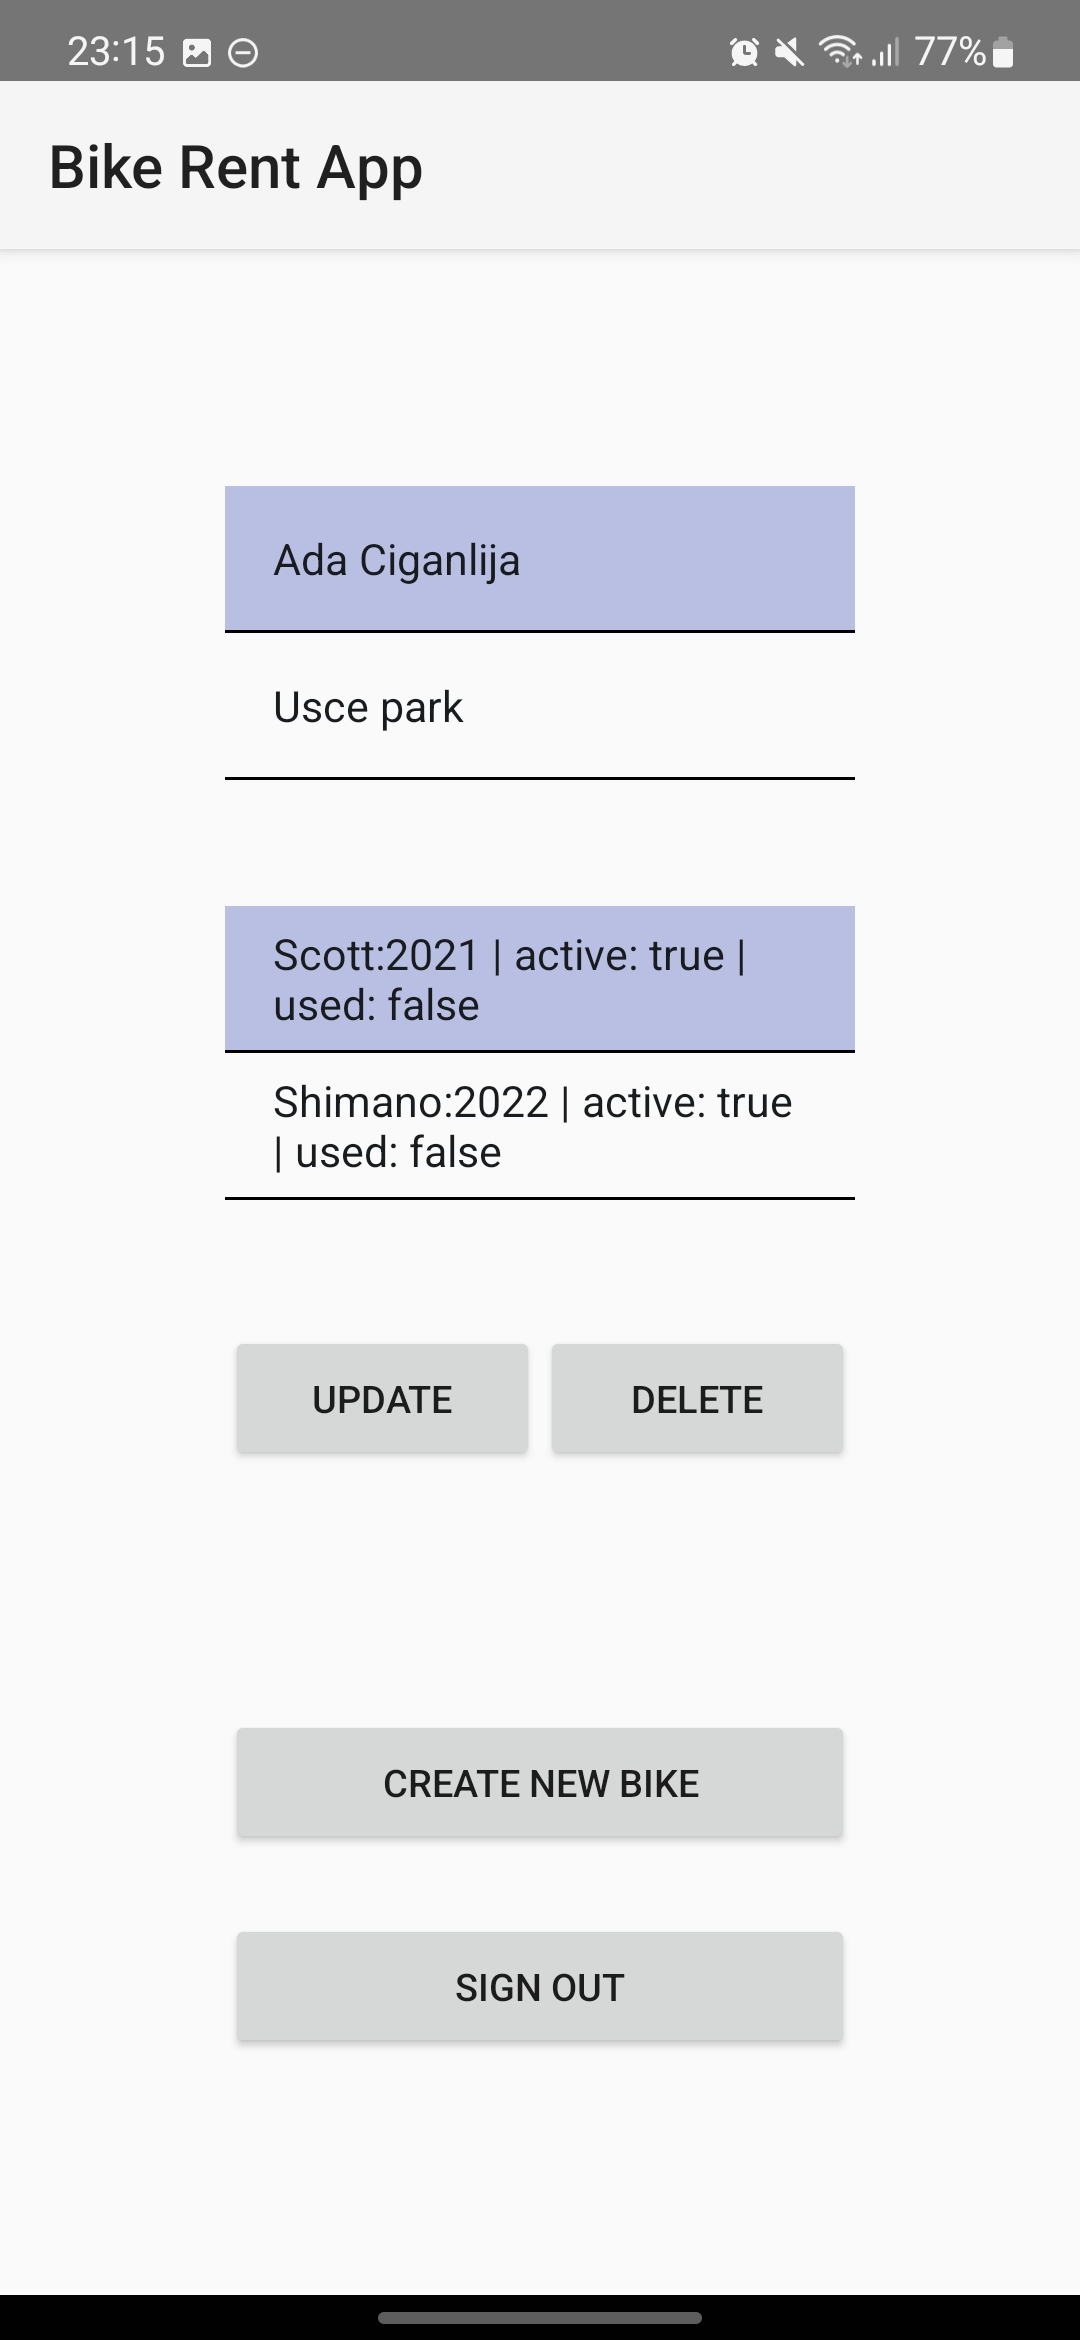
\includegraphics[height=0.6\textwidth]{Odabir bicikle za iznajmljivanje.jpg}
  % 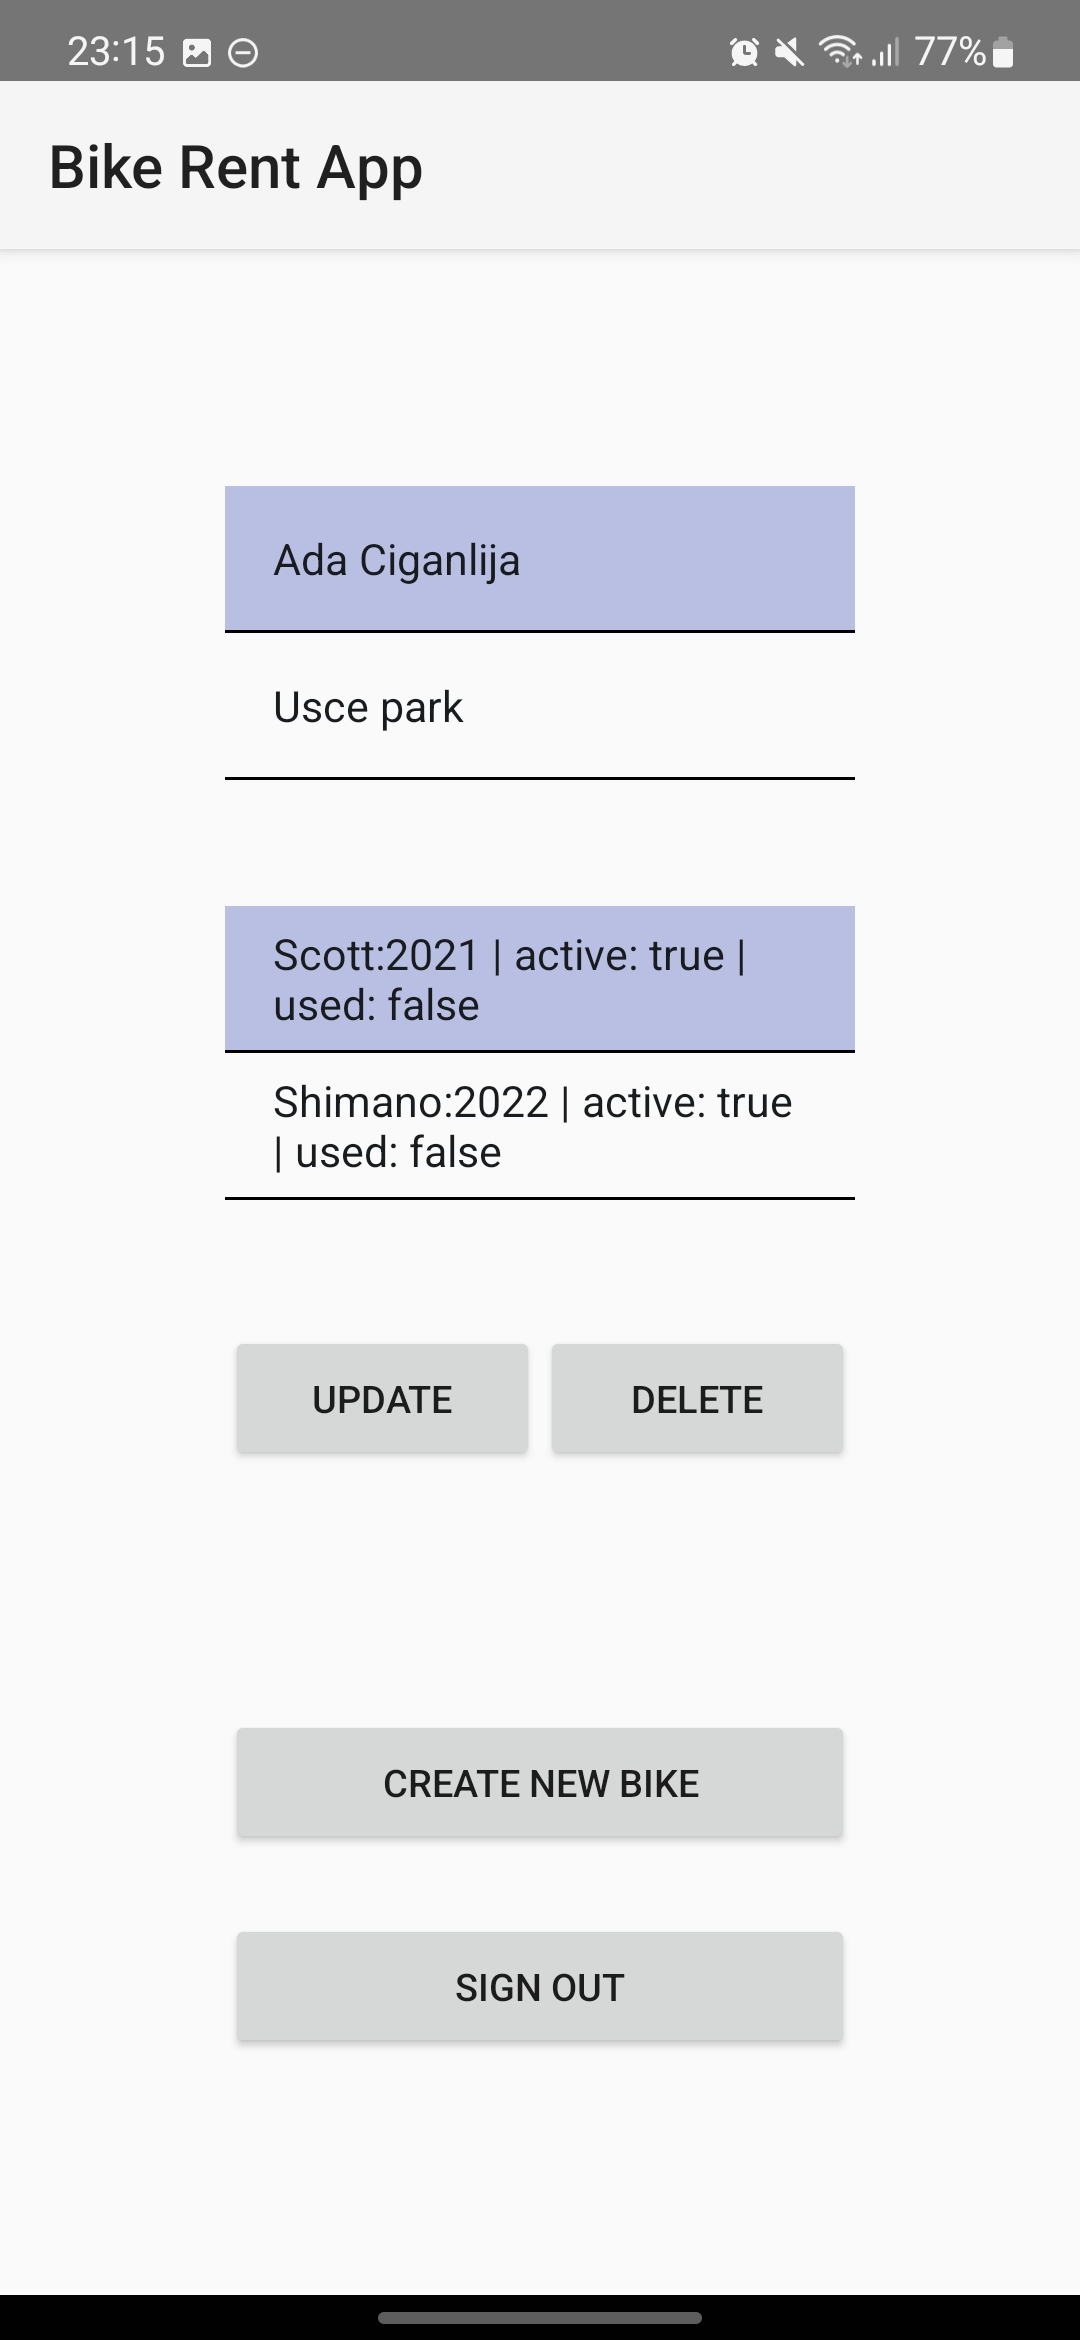
\includegraphics[width=0.7\textwidth]{Odabir bicikle za iznajmljivanje.jpg}
  \caption{Odabir bicikle za iznajmljivanje}
  \label{fig:odabirBicikle}
\end{figure}
 
\subsubsection{Upotreba aplikacije admin korisnika}

Kako servis koristi AWS Cognito servis za autentifikaciju i autorizaciju, proces registracije izvršava sam AWS Cognito servis. Svi korisnici imaju neverifikovan nalog dok ne potvrde email adresu posle registracije. Servis je konfiguirsan da se email koristi kao korisničko ime. Takođe uslovi koje šifra treba da zadovolji su postavljeni kada je konfigurisan servis. Na servisu je napravljena posebna grupa za admin korisnike. Da bi korisnik bio admin korisnik mora da zavodolji dva uslova. Prvi je da mora da ima verifikovan nalog a drugi je da mora ručno preko konzole da se dodeli admin grupi. Zbog organizacije AWS Cognito servisa, potrebno je vreme da se promena korisničke grupe propagira kroz sistem pa korisnik možda ne bude odmah svrstan u admin korisnike.
 

% TODO Kako ovo smanjiti?
\begin{figure}[!ht]
  \centering
  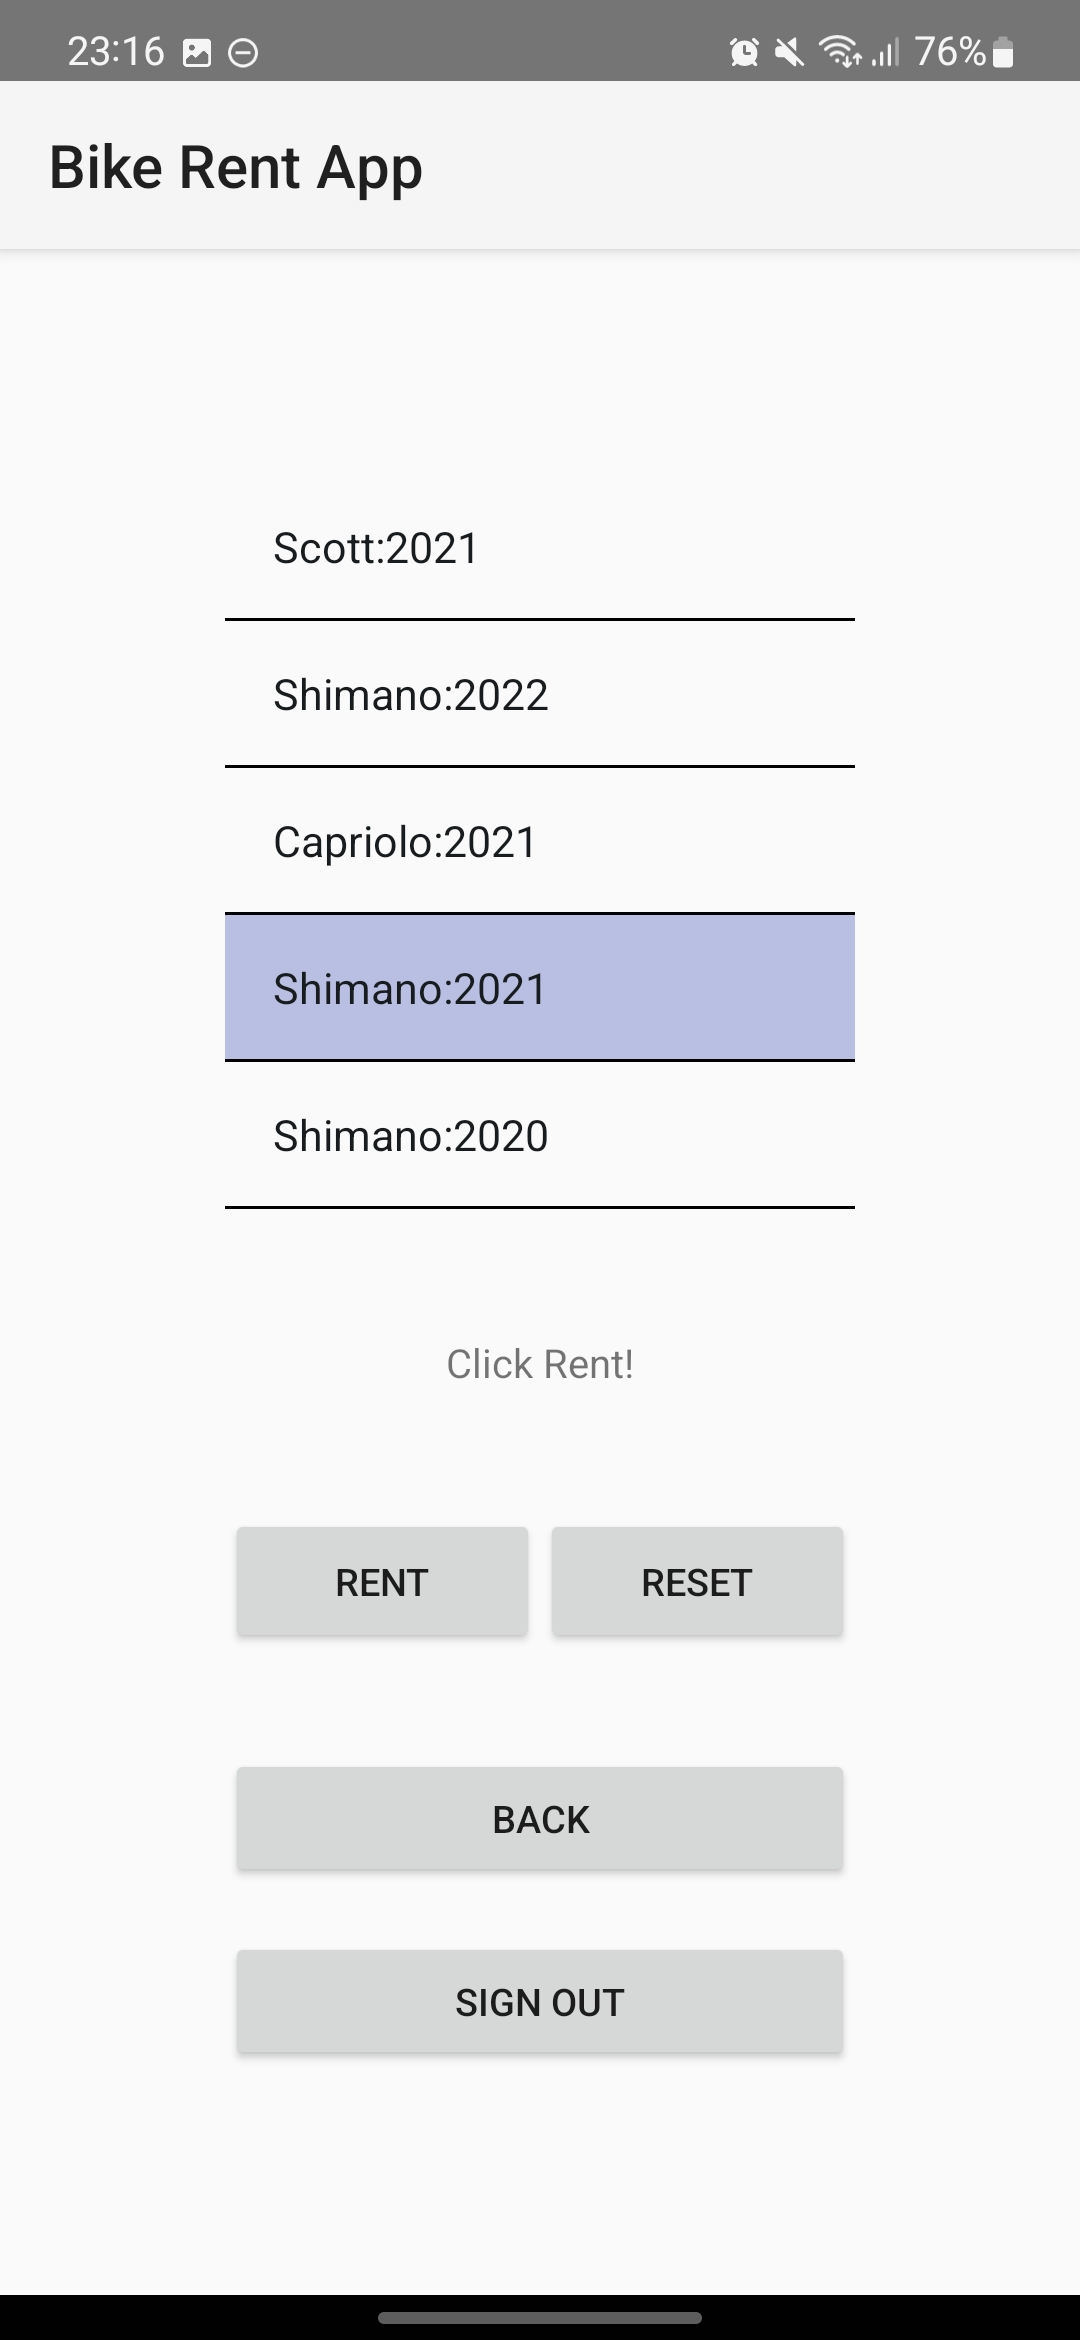
\includegraphics[height=0.6\textwidth]{AdminKorisnikInterfejs.jpg}
  % 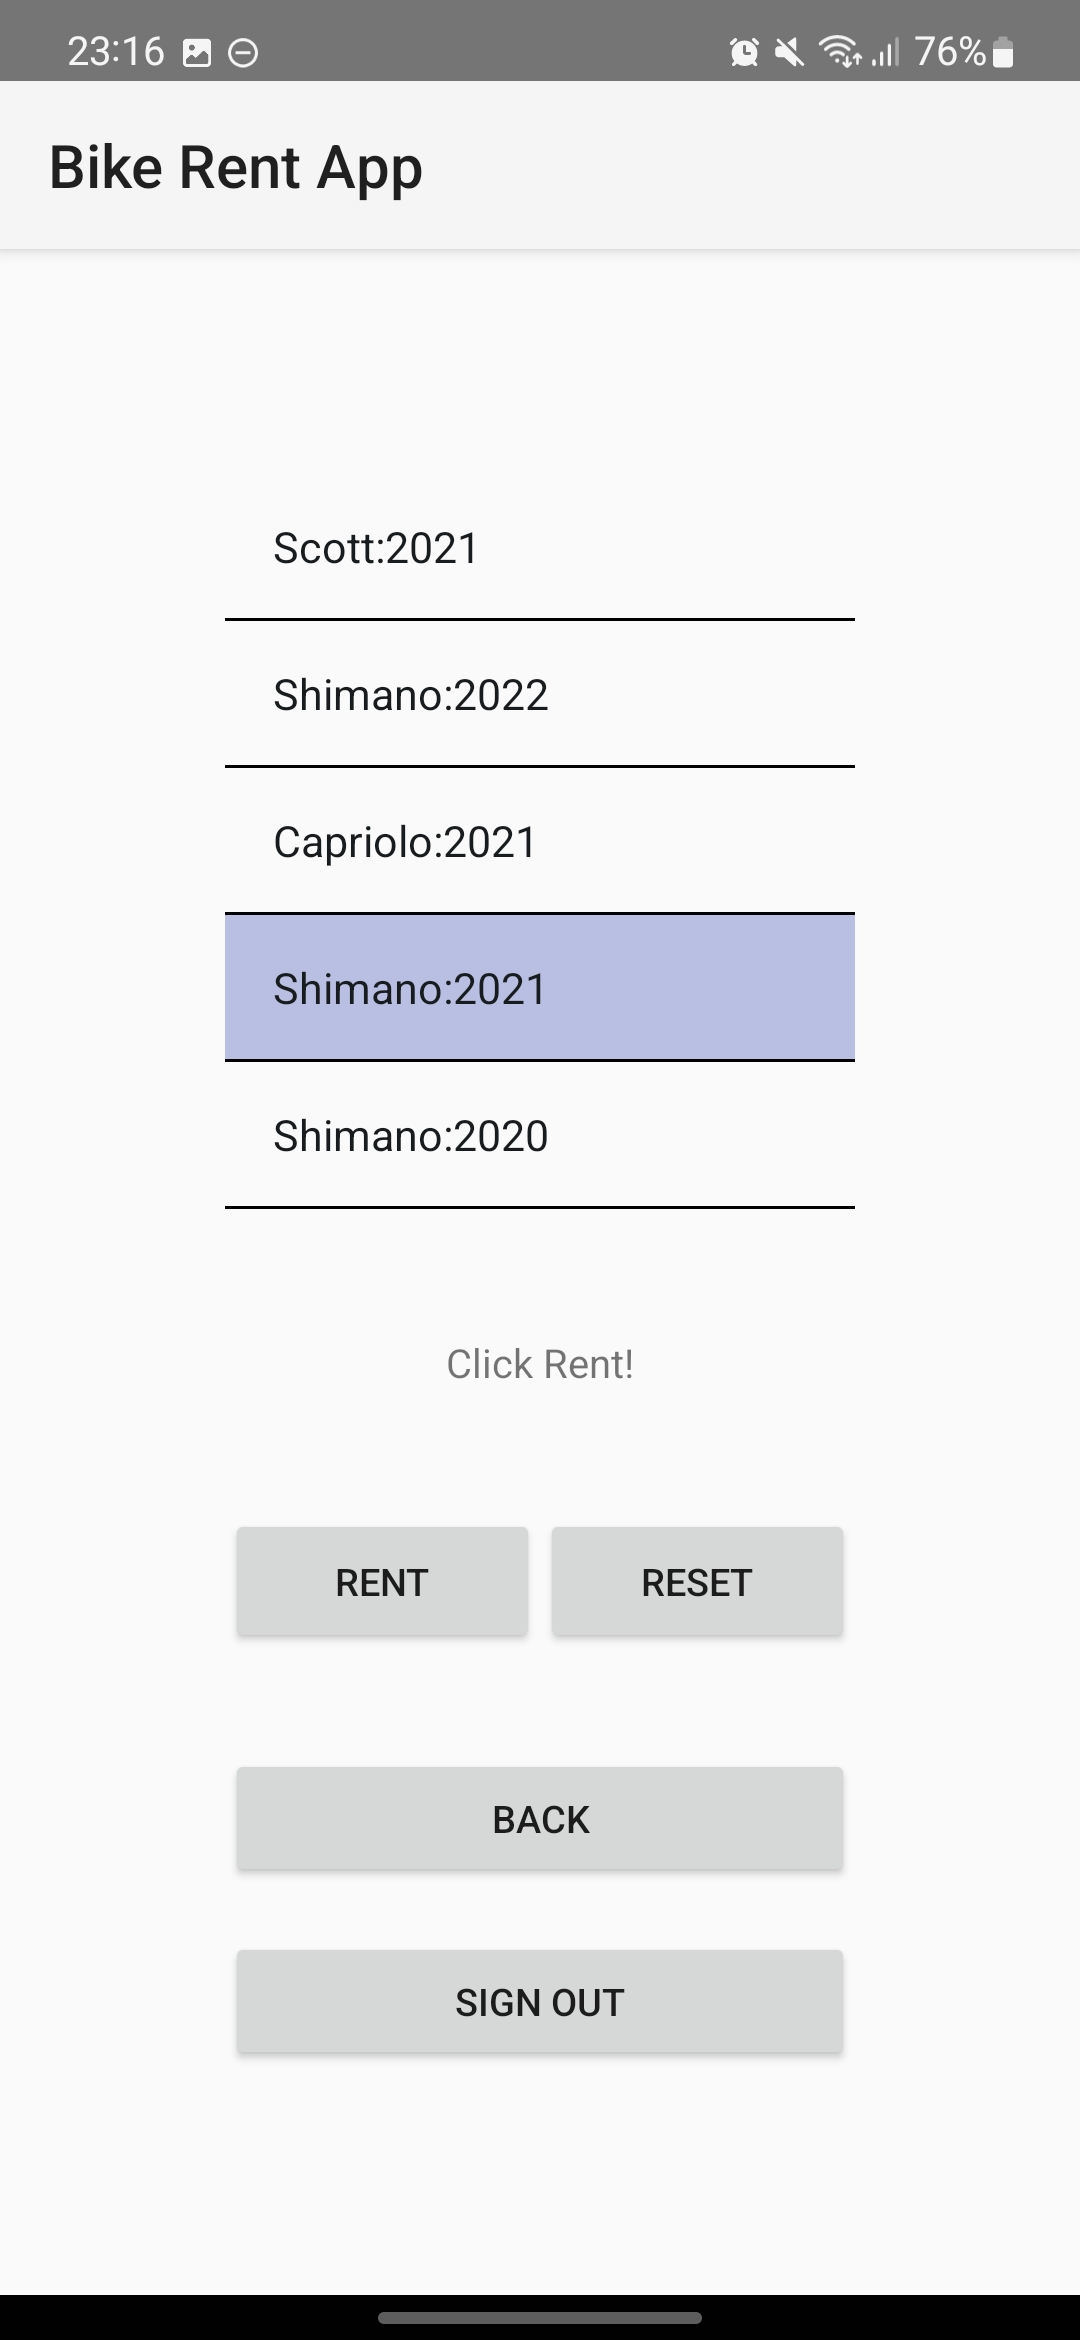
\includegraphics[width=0.7\textwidth]{AdminKorisnikInterfejs.jpg}
  \caption{Prikaz interfejsa admin korisnika}
  \label{fig:adminKorisnikInterfejs}
\end{figure}

 
Funkcionalnosti aplikacije korisnika koji je admin i regularnog korisnika se razlikuju. Regularan korisnik je u mogućnosti da iznajmljuje bicikle dok ta operacije nije omogućena admin korisniku. Nakon što se admin korisnik uloguje u aplikaciju na raspolaganje mu se stavlja izbor lokacije i opcija da doda novu biciklu u sistem. Ukoliko korisnik odabere lokaciju, aplikacija mu izlistava sve bicikle za tu lokaciju. To znači da admin korisnik može da vidi i bicikle koje u iznajmljene, one koje su deaktivirane i one koje su aktivne a ne iznajmljene. Ukoliko je bicikla deaktivirana to znači da neće biti stavljena na raspologanje regularnim korisnicima, niko neće moći da je iznajmi. Ova funkcionalnost je uvedena za slučaj da bicikla mora da ide u servis pa se ne može ponuditi korisniku. Odabirom bicikle, admin korisnik može da je aktivira, deaktivira ili obriše pritiskom na dugme. Važno je napomenuti da admin korisnik ne može da deaktivira ili obriše biciklu koju neko trenutno koristi i u slučaju da to pokuša, aplikacija vraća grešku. Kada jednom admin korisnik deaktivira biciklu, ona više neće biti stavljena na raspolaganje korisniku. Ukoliko pak admin korisnik obiše biciklu, servis je biriše iz baze pa više ni admin korisnik a ni regularni korisnik neće moći da je vidi kroz aplikaciju. Na slici\ref{fig:adminKorisnikInterfejs} se može videti primer interfejsa za admin korisnike.


Pored operacija aktiviranja, deaktiviranja i brisanja bicikle, admin korisniku se stavlja na raspolaganje i operacija kreiranja bicikle. Korisnik aktivira aktivnost pritiskom na drugme za kreiranje bicikle. Zatim se korisnik prebacuje na prozor\ref{fig:kreiranjeNovihBicikli} za kreiranje bicikle gde se traži da unese podatke o proizvođaču, godini proizvodnje, lokaciji. Aplikacija validira podatke i u slučaju da nisu uneta sva polja ili unosi nisu validni, aplikacija neće dozvoliti kreiranje bicikle i obavestiće korisnika koje polje treba da se promeni. Kada verifikacija prođe, aplikacija šalje zahtev servisu i korisnik se obaveštava o uspešnosti operacije. Na istom prozoru korisniku je omogućeno i da se vrati na prethodni ekran i prekine proces kreiranja bicikle. Takođe korisniku je omogućeno da se odjavi sa aplikacije pritiskom na dugme.
 
\begin{figure}[!ht]
  \centering
  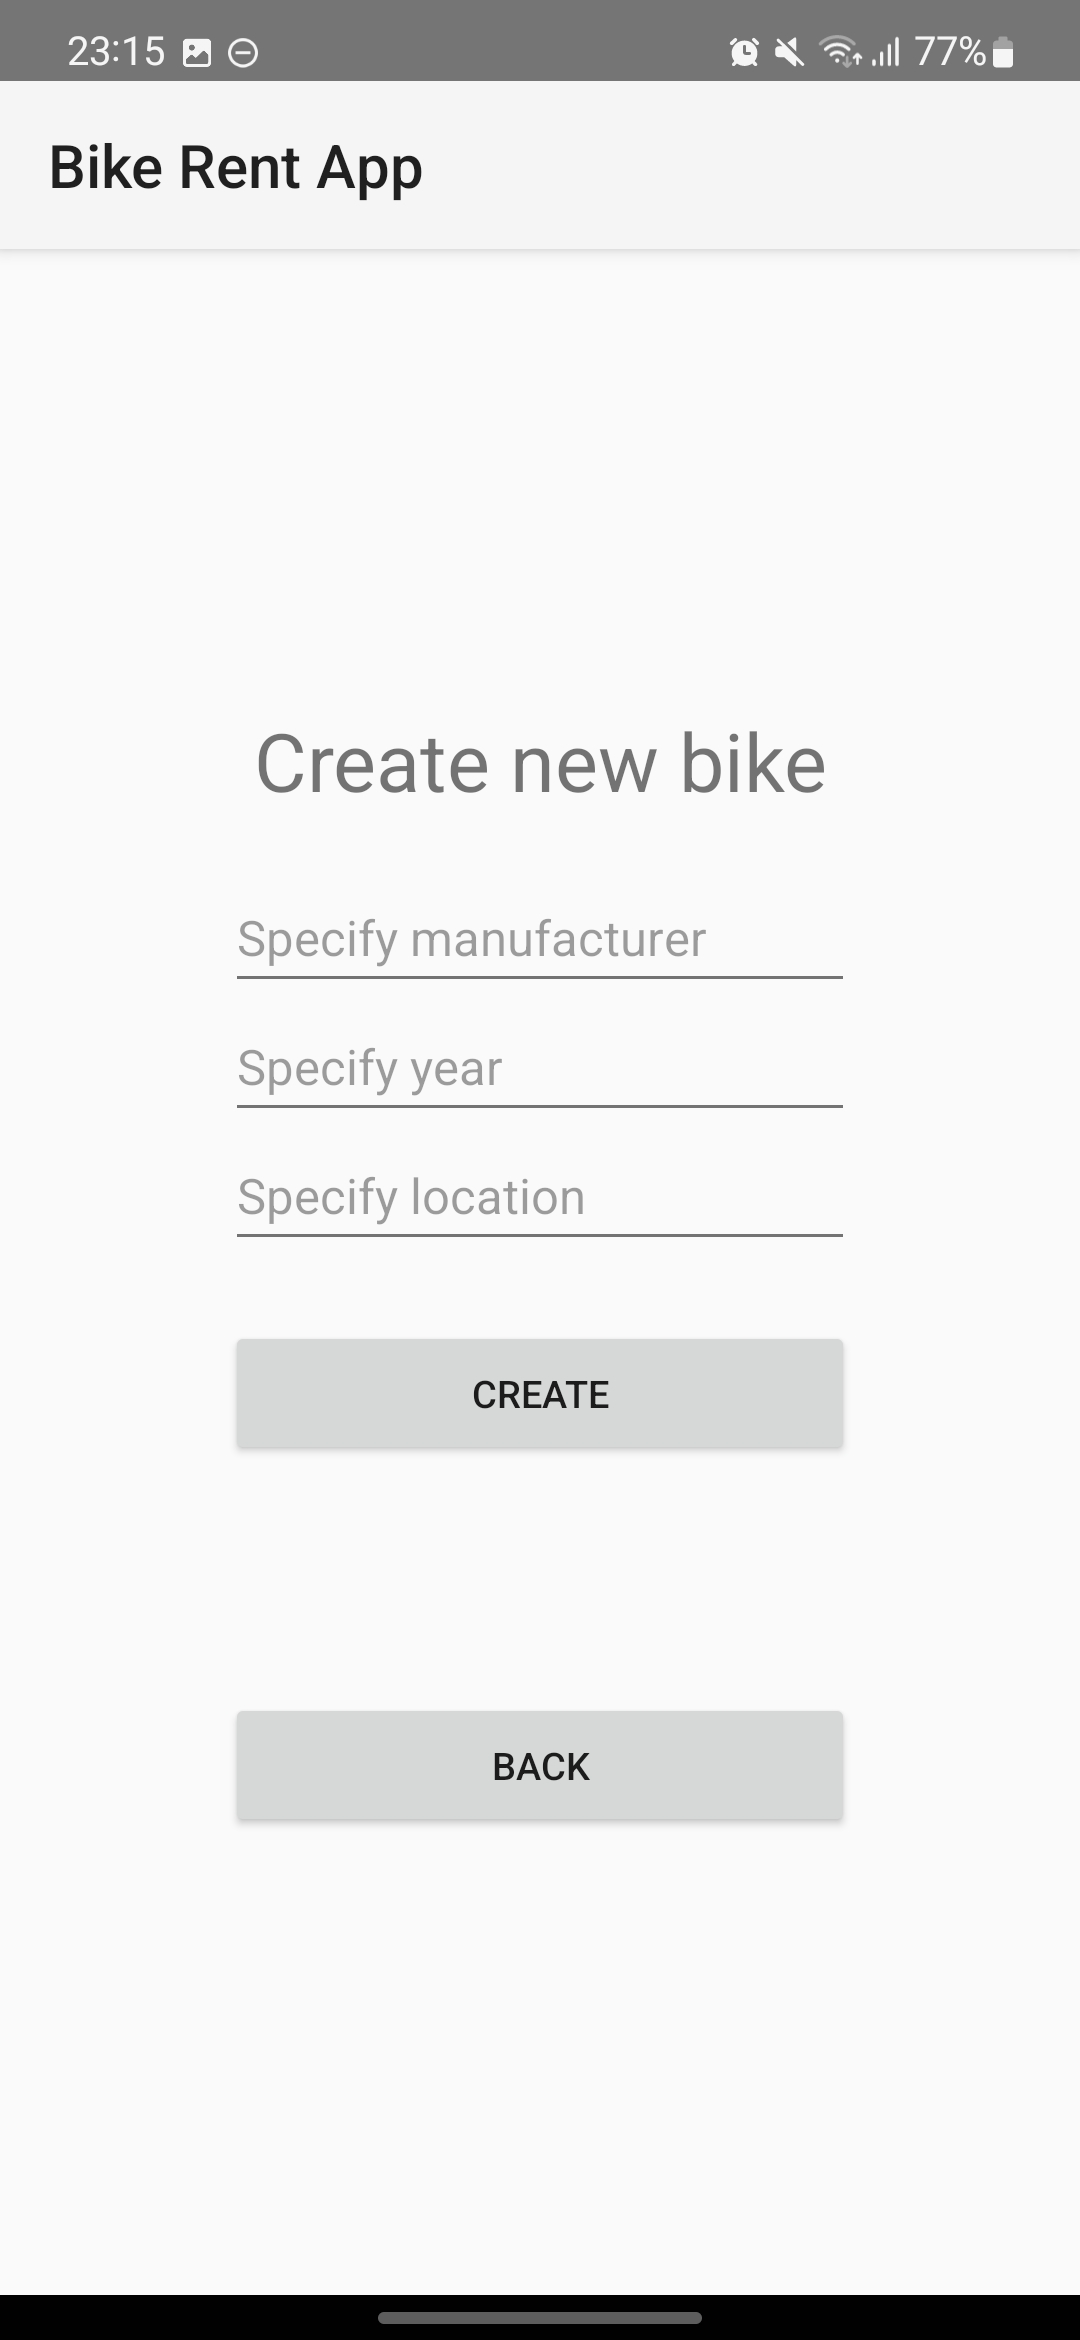
\includegraphics[height=0.6\textwidth]{Kreiranje nove bicikle.jpg}
  % 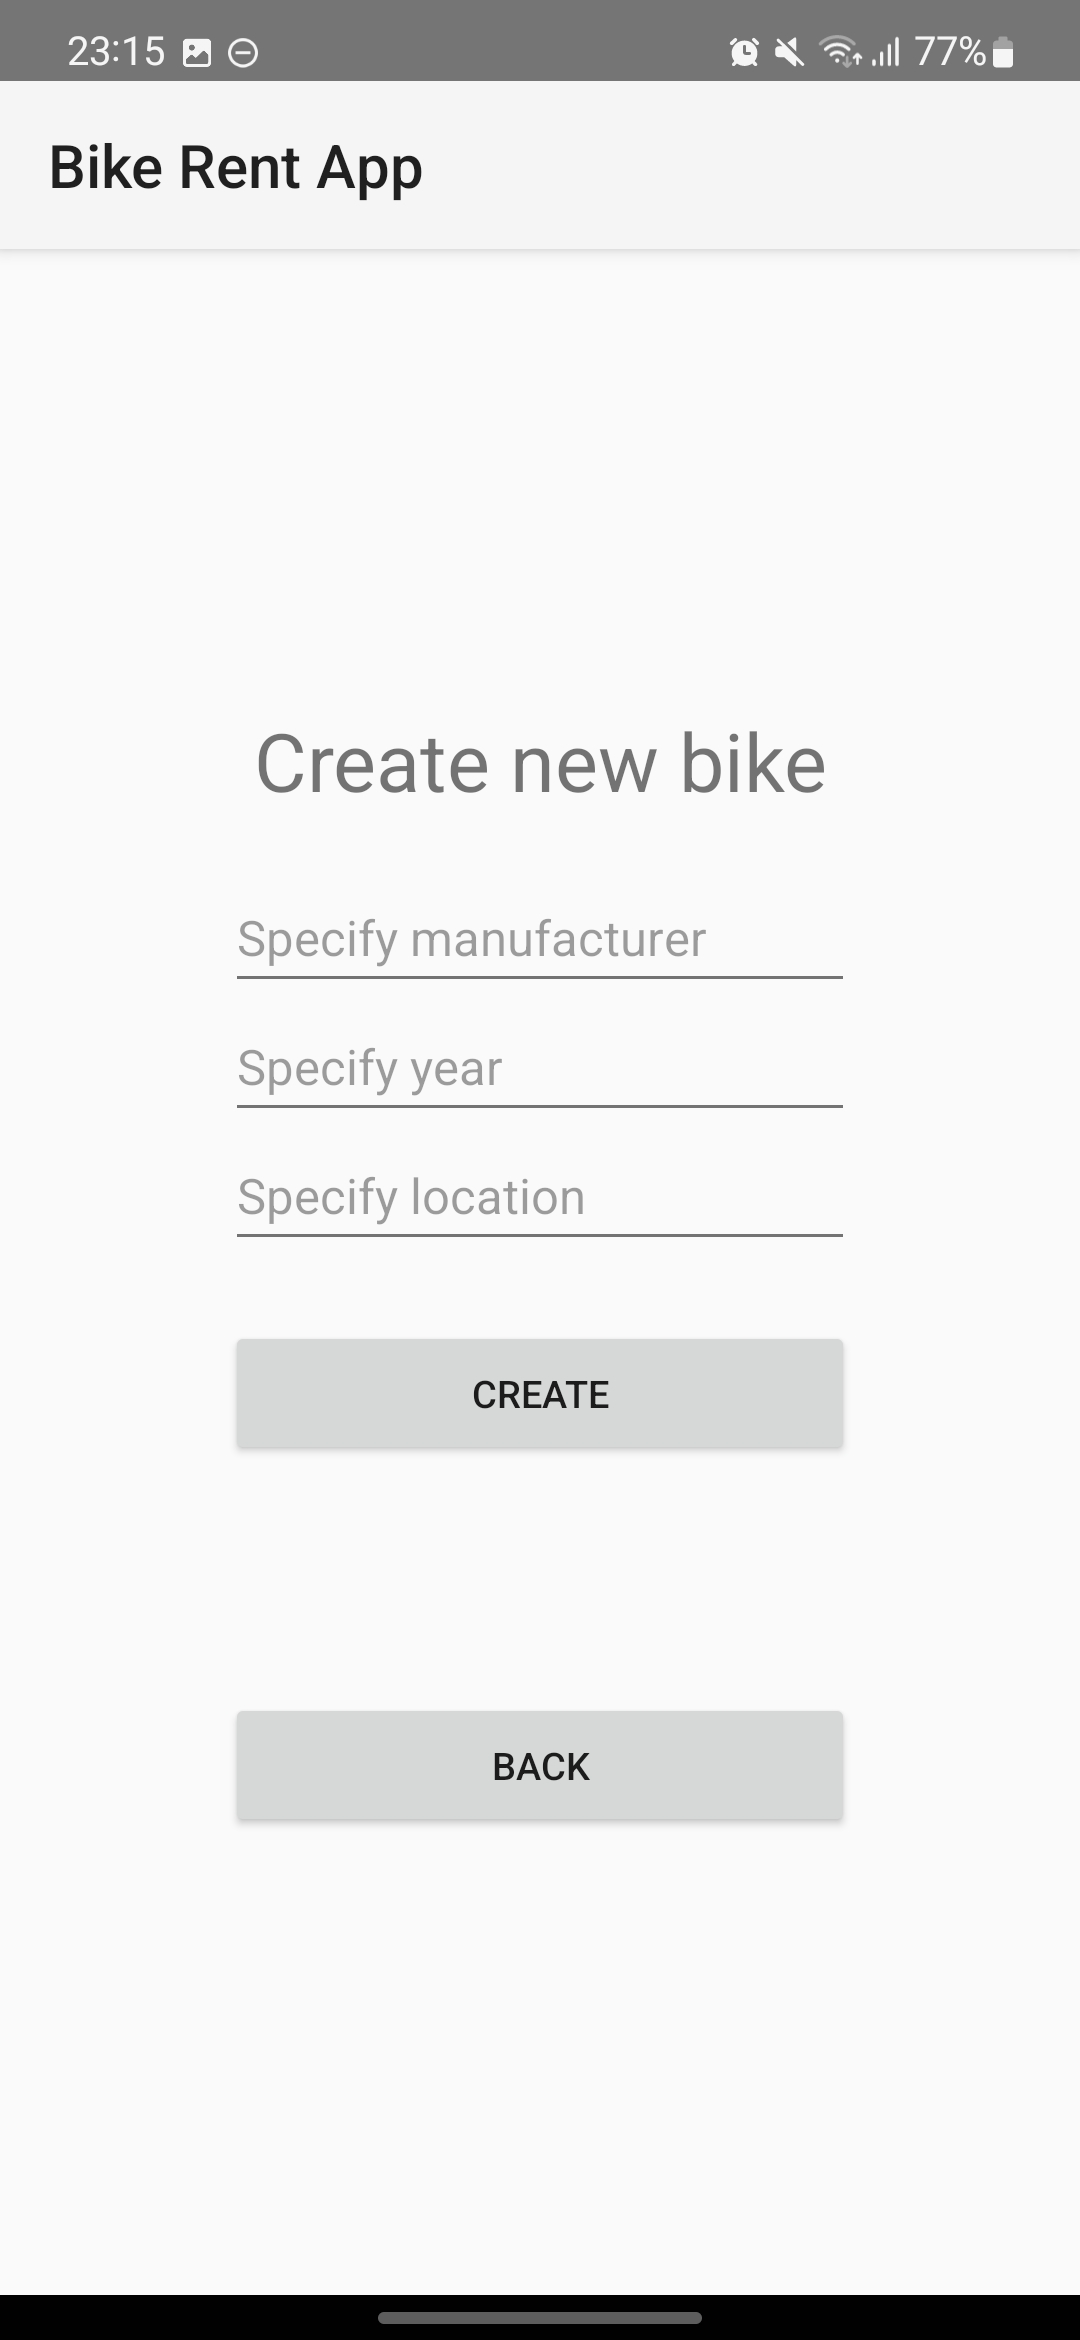
\includegraphics[width=0.7\textwidth]{Kreiranje nove bicikle.jpg}
  \caption{Prikaz interfjesa za kreiranje novih bicikli}
  \label{fig:kreiranjeNovihBicikli}
\end{figure}


% ------------------------------------------------------------------------------
\chapter{Zaključak}
% ------------------------------------------------------------------------------

U radu su prikazani ključni koncepti i tehnologije na kojima se zasniva razvoj softvera zasnovanog na arhitekturi bez servera. Raymotreni su i projektni uzorci softverske arhitekture kao i arhitekture bez servera. Opisani su prednosti i mane računarskih modela računarstva u oblaku sa posebnim fokusom na model funkcija kao usluga. Dalje je razmatran princip automatizovanja infrastrukture pod nazivom infrastruktura kao kod kao i serverles alat. Izrada softvera u skladu sa arhitekturom bez servera može doneti dosta benefita u vidu smanjenja troškova i količine operativnih zadataka kao i sposobnosti prilagođavanja promenama inteziteta dolaznog saobraćaja. Sa druge strane postoji vremensko organičenje izvršavanja operacije, spor odziv u nekim slučajevima kao i potencijalna zavisnost od pružaoca usluga. Arhitektura bez servera predstavlja jednu od alternativa klasičnom razvoju arhitekture sistema u oblaku.

U nastavku je detaljnije razmatran veb servisa koji je zasnovan na arhitekturi bez servera koji je razvijen u praktičnom delu projekta. Objasnjena je njegova arhitekturu kao i način upotrebe. Takođe obrađeni su i svi korišćeni servisi sa akcentom na AWS Lambda servis. Na kraju je razmotrena i android aplikacija koja je bila namenjena kao demonstracija klijentske aplikacije. Zajedno veb servis i aplikacija pružaju uvid na način razvoja aplikacija zasnovanih na arhitekturi bez servera. 

Pružaoci usluga svake godine proširuju funkcionalnosti servisa zasnovanih na računarstvu bez servera. U radu smo naveli i primere kompanija koje već uveliko koriste servise zasnovane na računarstvu bez servera. Mišljenje autora ovog rada je da će u narednom vremenu ovaj vid računarstva još više dobiti na značaju kako se više korisnika bude upoznalo sa tehnologiom.

% ------------------------------------------------------------------------------
% Literatura
% ------------------------------------------------------------------------------
\literatura

% ==============================================================================
% Završni deo teze i prilozi
\backmatter
% ==============================================================================

% ------------------------------------------------------------------------------
% Biografija kandidata
\begin{biografija}
  \textbf{Vojkan Cvijović} je rođen u Užicu 16. avgusta 1994. godine. Osnovnu i srednju škoklu je završio u Užicu. Osnovne studije na Matematičkom fakultetu, smer Infromatika, upisuje 2013. godine i završava 2017. kada upisuje i master studije na istom smeru. Od 2016. godine radi u multinacionalnoj kompaniji Endavi na razvoju platforme za isporučivanje okruženja u oblaku. Okruženje je zasnovano na virtuelnim mašinama i služi za pokretanje sistema za upravljanje sadržajem.
\end{biografija}
% ------------------------------------------------------------------------------

\end{document}
